\documentclass{beamer}

\usepackage[utf8]{inputenc}
\usepackage{minted}
\usepackage{tikz}
\usetikzlibrary{graphs,quotes,arrows.meta,positioning,shadows,calc,decorations.pathreplacing,fit}
\usepackage{graphicx}
\graphicspath{{figures/}}
\usepackage{pifont}
\usepackage{fontawesome5}
\usepackage{colortbl}
\usepackage{appendixnumberbeamer}
\usepackage[most]{tcolorbox}

\usetheme{Madrid}
\usecolortheme{seahorse}
% triangles instead of balls; plain numbers
\setbeamertemplate{itemize items}[triangle]
\setbeamertemplate{enumerate items}[default]
\setbeamertemplate{sections/subsections in toc}[default]
\setbeamertemplate{navigation symbols}{} % turn off navigation symbols

% Make hyperlinks blue
\hypersetup{
    colorlinks=true,
    urlcolor=blue!70,
    linkcolor=structure  % keep internal links using theme color
}

\setminted[julia]{fontsize=\footnotesize}
% every code block sits in a light rounded box (tcolorbox, no frame)
\tcbset{codebox/.style={enhanced, arc=1.5mm, boxrule=0pt, colback=gray!8, colframe=gray!8,
  left=3pt, right=3pt, top=1pt, bottom=1pt, boxsep=0pt, before skip=2pt, after skip=2pt}}
\BeforeBeginEnvironment{minted}{\begin{tcolorbox}[codebox]}
\AfterEndEnvironment{minted}{\end{tcolorbox}}

% Custom commands
\newcommand{\DFT}{\texttt{DataFlowTasks.jl}}
\newcommand{\cmark}{\ding{51}}%
\newcommand{\xmark}{\ding{55}}%

\newcommand\warning{%
 \makebox[1.4em][c]{%
 \makebox[0pt][c]{\raisebox{.1em}{\small!}}%
 \makebox[0pt][c]{\color{red}\Large$\bigtriangleup$}}}%

% Colors and pics from the 2023 DataFlowTasks slides
\definecolor{themegreen}{RGB}{0,100,0}
\definecolor{themelightgreen}{RGB}{230,239,230}
\definecolor{themelightblue}{RGB}{215,215,240}
\tikzset{
  pics/square/.default={1},
  pics/square/.style = {code = {\draw[pic actions] (0,0) rectangle (#1,#1);}}
}

% Small task graphs (Part 2): task = blue circle, dependency = gray arrow
\tikzset{
  dag/.style={font=\scriptsize},
  dnode/.style={draw, circle, fill=blue!25, minimum size=0.45cm, inner sep=0pt},
  dedge/.style={->, gray, thick},
}

% Task graph of a 3x3 tiled LU (used in Part 3); styles: lugraph, c (critical edges)
\tikzset{
  lugraph/.style={x=1.55cm, y=0.8cm, font=\scriptsize},
  lut/.style={draw, circle, minimum size=0.62cm, inner sep=0pt},
  lu/.style={lut, fill=themegreen!60},
  pan/.style={lut, fill=orange!60},
  up/.style={lut, fill=red!35},
  e/.style={->, gray},
  c/.style={->, very thick, structure},
}
\newcommand{\lugraph}{%
  % step 1
  \node[lu]  (L1)  at (0,0)    {11};
  \node[pan] (R12) at (1,1.5)  {12};
  \node[pan] (R13) at (1,0.5)  {13};
  \node[pan] (C21) at (1,-0.5) {21};
  \node[pan] (C31) at (1,-1.5) {31};
  \node[up]  (M22) at (2,1.5)  {22};
  \node[up]  (M23) at (2,0.5)  {23};
  \node[up]  (M32) at (2,-0.5) {32};
  \node[up]  (M33) at (2,-1.5) {33};
  % step 2
  \node[lu]  (L2)  at (3,1.5)  {22};
  \node[pan] (R23) at (4,1.0)  {23};
  \node[pan] (C32) at (4,0.0)  {32};
  \node[up]  (N33) at (5,-0.5) {33};
  % step 3
  \node[lu]  (L3)  at (6,-0.5) {33};
  % edges
  \foreach \a/\b in {L1/R12, L1/R13, L1/C31, R12/M22, R12/M32, R13/M23, R13/M33, C21/M23, C31/M32, C31/M33,
    M23/R23, M32/C32, L2/R23, R23/N33, M33/N33}
  	\draw[e] (\a) -- (\b);
  % critical path
  \foreach \a/\b in {L1/C21, C21/M22, M22/L2, L2/C32, C32/N33, N33/L3}
  	\draw[c] (\a) -- (\b);
}

% Timeline segment for TikZ: \tlseg{style}{start}{length}{row}{label} (x unit 0.55cm)
\newcommand{\tlseg}[5]{\node[#1, minimum width=#3*0.55cm] at (#2,#4) {#5};}

% visible on=<overlay>: draw a TikZ element only on some slides (keeps the bounding box)
\tikzset{
  invisible/.style={opacity=0, text opacity=0},
  visible on/.style={alt={#1{}{invisible}}},
  alt/.code args={<#1>#2#3}{\alt<#1>{\pgfkeysalso{#2}}{\pgfkeysalso{#3}}},
}

% Task timeline styles: running on a thread / runnable (waiting for a thread) / blocked (waiting for I/O)
\tikzset{
  tl/.style={draw, minimum height=0.32cm, inner sep=0pt, anchor=west, font=\tiny},
  running/.style={tl, fill=blue!30},
  runnable/.style={tl, fill=orange!25, draw=orange!60},
  blocked/.style={tl, fill=gray!15, draw=gray!60, dashed},
}

% Root of the demo links: latexmkrc sets an absolute file:// URL (works in Skim);
% the default, relative run: links, work in Okular/Acrobat after cloning the repo.
\providecommand{\demoroot}{run:../}
% --- Boxes (tcolorbox) -------------------------------------------------------
% common look: rounded frame in color #1, light fill
\tcbset{talk/.style={enhanced, arc=1.5mm, boxrule=0.6pt, colframe=#1, colback=#1!10},
        talk/.default=structure}
% badge: small box on the line, \badge[color]{text}
\newtcbox{\badge}[1][structure]{talk=#1, on line, arc=1mm, boxsep=1pt,
  left=2pt, right=2pt, top=0.5pt, bottom=0.5pt, fontupper=\footnotesize\bfseries}
% punchline: centered, hugs its text
\NewTotalTCBox{\punchline}{m}{talk, hbox, center, boxsep=2pt, left=4pt, right=4pt}{#1}
% hands-on checkpoint: \yourturn{minutes}{what to do}
\NewTColorBox{yourturnbox}{m}{talk=red!70!black, fonttitle=\bfseries\small,
  title={\faKeyboard\ Your turn (\(\sim\)#1 min)}, boxsep=2pt, top=1pt, bottom=1pt}
\newcommand{\yourturn}[2]{\begin{yourturnbox}{#1}#2\end{yourturnbox}}
% recurring cue linking a primitive to its use inside DataFlowTasks.jl
\NewTotalTCBox{\indft}{m}{talk=themegreen, boxsep=2pt, top=1pt, bottom=1pt, fontupper=\small}
  {\faLink\ \textbf{In \DFT:} #1}

% Corner badges, fixed position: bottom-right, just above the footline
\newcommand{\cornerbadge}[1]{%
  \begin{tikzpicture}[remember picture, overlay]
    \node[anchor=south east, inner sep=0pt] at ($(current page.south east)+(-0.25cm,0.55cm)$) {#1};
  \end{tikzpicture}%
}
% clickable live demo link (opens the file in ../scripts): \livedemobox{color}{label}{file}
\newcommand{\livedemobox}[3]{%
  \cornerbadge{\href{\demoroot scripts/#3}{\badge[#1]{\faCode\ #2: \texttt{\detokenize{#3}}}}}}
\newcommand{\livedemo}[1]{\livedemobox{structure}{Live demo}{#1}}
% optional demo: skip if short on time
\newcommand{\livedemoopt}[1]{\livedemobox{gray}{Optional demo}{#1}}
% live demo typed in the REPL (no script)
\newcommand{\livedemorepl}{\cornerbadge{\badge{\faTerminal\ Live demo: REPL}}}
% hands-on file (in ../handson)
\newcommand{\handson}[1]{%
  \cornerbadge{\href{\demoroot handson/#1}{\badge[themegreen]{\faCode\ Hands-on: \texttt{\detokenize{handson/#1}}}}}}
% skippable frame: small tag in the top-right corner (skip if running late)
\newcommand{\skippable}{%
  \begin{tikzpicture}[remember picture, overlay]
    \node[anchor=north east, font=\tiny\color{gray}, inner sep=2pt]
      at ($(current page.north east)+(-0.2cm,-0.75cm)$) {skippable};
  \end{tikzpicture}%
}

\AtBeginSection[]
{
  \begin{frame}
    \frametitle{Table of Contents}
    \tableofcontents[currentsection]
    \addtocounter{framenumber}{-1}
  \end{frame}
}
% signpost between subsections (the first one follows the section TOC)
\AtBeginSubsection[]
{
  \ifnum\value{subsection}>1
  \begin{frame}
    \frametitle{Table of Contents}
    \tableofcontents[currentsection, currentsubsection]
    \addtocounter{framenumber}{-1}
  \end{frame}
  \fi
}

%Information to be included in the title page:
\title[Shared memory parallelism]
{Shared memory parallelism in Julia}
\subtitle{Tasks, threads, and \DFT}

\author{Luiz~M.~Faria}

\institute[POEMS]{ANF Julia4HPC, Fréjus}

\date{13 October 2026}

\titlegraphic{
    
\includegraphics[height=0.8cm]{poems-logo.png}         \quad
    
\includegraphics[height=0.8cm]{inr_logo_grisbleu.png}  \quad
    
\includegraphics[height=0.8cm]{cnrs-logo.png} \quad
    
\includegraphics[height=0.8cm]{Logo_ENSTA_Paris.jpg}
}

\begin{document}

\begin{frame}[plain]
	\titlepage
\end{frame}


\begin{frame}
	\frametitle{Roadmap}
	\begin{itemize}
		\item \textbf{13:30--14:50 \textperiodcentered{} Multithreading in Julia}
		      \begin{itemize}
			      \item Tasks and threads
			      \item Independent iterations: chunks, buffers, data races, locks, atomics
			      \item Dependent tasks: \texttt{wait}, fork-join, last writers
		      \end{itemize}
		      \medskip
		\item \textbf{15:10--16:00 \textperiodcentered{} \DFT}
		      \begin{itemize}
			      \item Task dependencies inferred from data
			      \item Under the hood: the Part~1 primitives
			      \item Tiled LU again, and profiling
		      \end{itemize}
		      \medskip
		\item \textbf{16:00--17:30 \textperiodcentered{} Hands-on project}
		      \begin{itemize}
			      \item Explore the scripts, bring your own code, or a project
		      \end{itemize}
	\end{itemize}
\end{frame}

% ---------------------------------------------------------------------------
\begin{frame}[fragile]
	\frametitle{Setup: do it now}
	\begin{enumerate}
		\item Clone the repository
		      \begin{minted}[fontsize=\footnotesize]{text}
$ git clone https://github.com/maltezfaria/2026-frejus
$ cd 2026-frejus
		      \end{minted}
		\item Install the packages (\DFT, GraphViz, GLMakie, BenchmarkTools)
		      \begin{minted}[fontsize=\footnotesize]{text}
$ julia --project -e 'using Pkg; Pkg.instantiate()'
		      \end{minted}
		      {\small Precompiling takes a few minutes: let it run while we start}
		\item Start Julia with threads
		      \begin{minted}[fontsize=\footnotesize]{text}
$ julia --project -t auto
		      \end{minted}
	\end{enumerate}

	\vfill
	\punchline{Part~1 needs only \texttt{Base}: no need to wait for step~2}
\end{frame}

\section{Multithreading in Julia}
\subsection{Tasks and threads}

\begin{frame}
	\frametitle{Parallel computing in Julia}
	\alert{Four} kinds of concurrent/parallel programming:
	\medskip

	\centering\small
	\renewcommand{\arraystretch}{1.3}
	\setlength{\tabcolsep}{4pt}
	\begin{tabular}{l l l l}
		\textbf{Paradigm}     & \textbf{Memory} & \textbf{Julia tools}                             & \textbf{When} \\
		\hline
		\rowcolor{structure!10}
		Asynchronous tasks    & shared          & \texttt{Task}, \texttt{Channel}, \ldots          & \alert{today} \\
		\rowcolor{structure!10}
		Multi-threading       & shared          & \texttt{@threads}, \texttt{@spawn}, locks     & \alert{today} \\
		GPU computing         & device          & \texttt{CUDA.jl}, \texttt{AMDGPU.jl}, \ldots     & Wednesday     \\
		Distributed computing & distributed     & \texttt{Distributed}, \texttt{MPI.jl}, \ldots    & Friday        \\
	\end{tabular}

	\vfill
	\begin{tikzpicture}[
			x=1cm, y=1cm, font=\scriptsize,
			mem/.style={draw, fill=green!15, minimum height=0.35cm, inner sep=1pt},
			core/.style={draw, fill=orange!30, minimum size=0.3cm, inner sep=0pt},
			link/.style={-, thick, gray},
		]
		% --- Shared memory ---
		\fill[structure!10, rounded corners] (-0.2,-0.75) rectangle (3.0,1.25);
		\node[mem, minimum width=2.6cm] (ram) at (1.4,0.8) {memory};
		\foreach \i in {0,...,3} {
				\node[core] (c\i) at ({0.35+0.7*\i},0) {};
				\draw[link] (c\i) -- (c\i |- ram.south);
			}
		\node at (1.4,-0.5) {\textbf{shared}: threads, tasks};

		% --- GPU ---
		\begin{scope}[xshift=3.6cm]
			\node[mem, minimum width=1.0cm] (hram) at (0.5,0.8) {RAM};
			\node[core] (hcpu) at (0.5,0) {};
			\draw[link] (hcpu) -- (hram);
			\node[mem, minimum width=1.2cm] (vram) at (2.5,0.8) {VRAM};
			\foreach \i in {0,...,4} {
					\node[core, fill=red!25, minimum size=0.15cm] (g\i) at ({2.1+0.2*\i},0) {};
					\draw[link, thin] (g\i) -- (g\i |- vram.south);
				}
			\draw[<->, thick] (hram) -- node[above] {copy} (vram);
			\node at (1.5,-0.5) {\textbf{device}: GPU};
		\end{scope}

		% --- Distributed ---
		\begin{scope}[xshift=7.5cm]
			\foreach \i in {0,...,2} {
					\node[mem, minimum width=0.8cm] (m\i) at ({0.5+1.1*\i},0.8) {mem};
					\node[core] (p\i) at ({0.5+1.1*\i},0) {};
					\draw[link] (p\i) -- (m\i);
					\draw[link] (p\i) -- ++(0,-0.2);
				}
			\draw[thick, dashed] (0.5,-0.2) -- (2.7,-0.2);
			\node at (1.6,-0.5) {\textbf{distributed}: messages};
		\end{scope}

	\end{tikzpicture}

	\medskip
	\begin{tabular}{l}
		\textcolor{green!50!black}{\cmark} \textbf{No explicit communication}                \\
		\textcolor{red}{\xmark} \textbf{Synchronization is your job} (\alert{data races!}) \\
	\end{tabular}

	% \vfill
	% \begin{flushright}
	% 	\footnotesize\url{https://docs.julialang.org/en/v1/manual/parallel-computing/}
	% \end{flushright}
\end{frame}

% ---------------------------------------------------------------------------
\begin{frame}[fragile]
	\frametitle{What is a task?}
	\textbf{Task:} a unit of work that can be \alert{suspended} and \alert{resumed}\\
	\textcolor{gray}{\small a.k.a.\ coroutine, lightweight thread}

	\vfill
	\begin{columns}[c]
		\column{0.62\textwidth}
		\begin{minted}{julia}
f = () -> (sleep(1); 1 + 1)

t = Task(f)  # create
schedule(t)  # start: returns at once
fetch(t)     # wait 1 s, get result
# 2
		\end{minted}

		\column{0.36\textwidth}
		\centering
		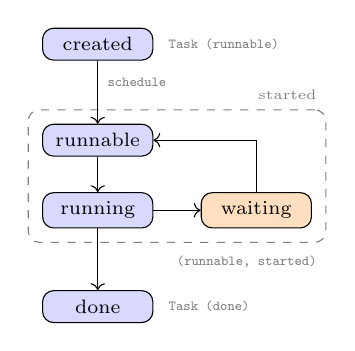
\begin{tikzpicture}[
				font=\scriptsize, node distance=0.45cm and 0.5cm,
				st/.style={draw, rounded corners, fill=blue!15, minimum width=1.4cm, minimum height=0.4cm},
				lab/.style={font=\tiny\ttfamily, text=gray},
			]
			\node[st] (cr) {created};
			\node[st, below=0.8cm of cr] (rn) {runnable};
			\node[st, below=of rn] (ru) {running};
			\node[st, right=0.6cm of ru, fill=orange!25] (wt) {waiting};
			\node[draw=gray, dashed, rounded corners, inner sep=5pt,
				fit=(rn) (ru) (wt)] (started) {};
			\node[st, below=0.6cm of started.south -| ru] (dn) {done};
			\node[font=\tiny, text=gray, anchor=south east] at (started.north east) {started};
			\draw[->] (cr) -- node[right, lab, pos=0.35] {schedule} (rn);
			\draw[->] (rn) -- (ru);
			\draw[->] (ru) -- (dn);
			\draw[->] (ru) -- (wt);
			\draw[->] (wt) |- (rn);
			% what the REPL prints
			\node[lab, right=2pt of cr] {Task (runnable)};
			\node[lab, below=1pt of started.south east, anchor=north east] {(runnable, started)};
			\node[lab, right=2pt of dn] {Task (done)};
		\end{tikzpicture}
	\end{columns}

	\vfill
	Syntactic sugar:
	\begin{minted}{julia}
t = @task f()   # Task(f)
t = @async f()  # Task + schedule: current thread (discouraged)
t = @spawn f()  # Task + t.sticky = false + schedule: any thread
	\end{minted}

	\livedemorepl
\end{frame}

% ---------------------------------------------------------------------------
\begin{frame}[fragile]
	\frametitle{Example: concurrency}
	\textbf{I/O-bound}: 20 queries to \alert{HAL}, \alert{single thread} (\texttt{julia -t 1})

	\medskip
	\begin{minted}{julia}
using Downloads: download
api = "https://api.archives-ouvertes.fr/search"
# HAL publications of a given year
hal(year) = "$api/?q=producedDateY_i:$year"
urls = hal.(2005:2024)

@time map(download, urls)                          # 2.8 s
@time fetch.(map(u -> @spawn(download(u)), urls))  # 0.2 s
	\end{minted}
	Waiting for the network \alert{suspends} the task \(\Rightarrow\) the thread runs another one

	\vfill
	\centering
	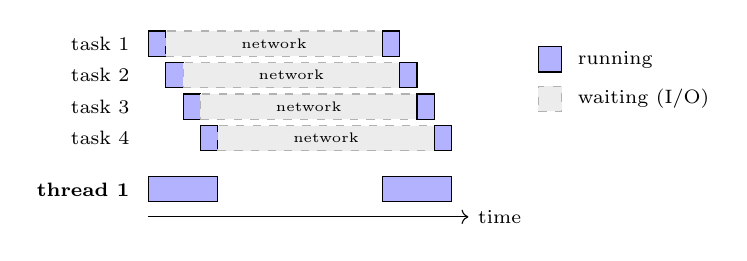
\begin{tikzpicture}[x=0.55cm, y=1cm, font=\scriptsize]
		\foreach \k in {0,...,3} {
				\node[anchor=east] at (-0.2,-0.4*\k) {task \the\numexpr\k+1};
				\tlseg{running}{0.4*\k}{0.4}{-0.4*\k}{}
				\tlseg{blocked}{0.4*\k+0.4}{5}{-0.4*\k}{network}
				\tlseg{running}{0.4*\k+5.4}{0.4}{-0.4*\k}{}
			}
		\node[anchor=east] at (-0.2,-1.85) {\textbf{thread 1}};
		\tlseg{running}{0}{1.6}{-1.85}{}
		\tlseg{running}{5.4}{1.6}{-1.85}{}
		\draw[->] (0,-2.2) -- (7.4,-2.2) node[right] {time};
		% legend
		\node[running, minimum width=0.3cm] at (9,-0.2) {}; \node[anchor=west] at (9.7,-0.2) {running};
		\node[blocked, minimum width=0.3cm] at (9,-0.7) {}; \node[anchor=west] at (9.7,-0.7) {waiting (I/O)};
	\end{tikzpicture}

	\livedemo{concurrency.jl}
\end{frame}

% ---------------------------------------------------------------------------
\begin{frame}[fragile]
	\frametitle{Example: no concurrency gain}
	\textbf{CPU-bound}: factor 10 matrices, \alert{single thread} (\texttt{julia -t 1})

	\medskip
	\begin{minted}{julia}
using LinearAlgebra
BLAS.set_num_threads(1)  # more on this later
As = [rand(2000, 2000) for _ in 1:10]

@time map(lu, As)                          # 1.1 s
@time fetch.(map(A -> @spawn(lu(A)), As))  # 1.1 s
	\end{minted}

	\vfill
	\centering
	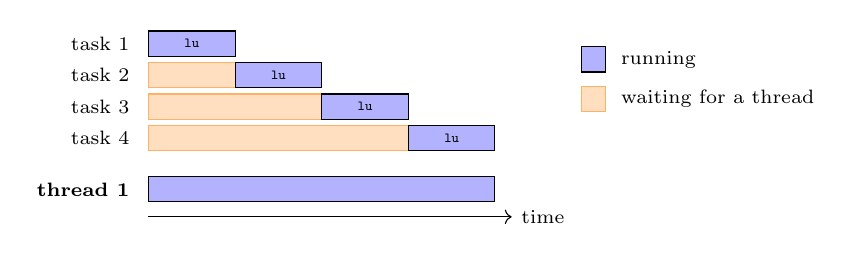
\begin{tikzpicture}[x=0.55cm, y=1cm, font=\scriptsize]
		\foreach \k in {0,...,3} {
				\node[anchor=east] at (-0.2,-0.4*\k) {task \the\numexpr\k+1};
				\ifnum\k>0 \tlseg{runnable}{0}{2*\k}{-0.4*\k}{} \fi
				\tlseg{running}{2*\k}{2}{-0.4*\k}{\texttt{lu}}
			}
		\node[anchor=east] at (-0.2,-1.85) {\textbf{thread 1}};
		\tlseg{running}{0}{8}{-1.85}{}
		\draw[->] (0,-2.2) -- (8.4,-2.2) node[right] {time};
		% legend
		\node[running, minimum width=0.3cm] at (10,-0.2) {}; \node[anchor=west] at (10.7,-0.2) {running};
		\node[runnable, minimum width=0.3cm] at (10,-0.7) {}; \node[anchor=west] at (10.7,-0.7) {waiting for a thread};
	\end{tikzpicture}

	\vfill
	\raggedright
	\begin{itemize}
		\item \alert{Cooperative}: a task gives its thread back only when it \textbf{waits} or \textbf{finishes}, and \texttt{lu} never waits
	\end{itemize}

	\livedemo{parallelism.jl}
\end{frame}


% ---------------------------------------------------------------------------
\begin{frame}[fragile]
	\frametitle{Same code, more threads}
	\textbf{CPU-bound}: factor 10 matrices, \alert{four threads} (\texttt{julia -t 4})

	\medskip
	\begin{minted}{julia}
@time map(lu, As)                          # 1.1 s
@time fetch.(map(A -> @spawn(lu(A)), As))  # 0.4 s
	\end{minted}

	\vfill
	\centering
	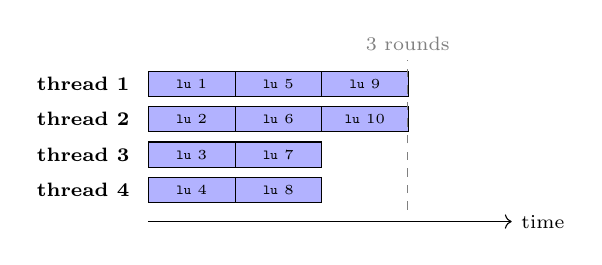
\begin{tikzpicture}[x=0.55cm, y=1cm, font=\scriptsize]
		\foreach \th in {0,...,3} {
				\node[anchor=east] at (-0.2,-0.45*\th) {\textbf{thread \the\numexpr\th+1}};
				\tlseg{running}{0}{2}{-0.45*\th}{\texttt{lu} \the\numexpr\th+1}
				\tlseg{running}{2}{2}{-0.45*\th}{\texttt{lu} \the\numexpr\th+5}
			}
		\tlseg{running}{4}{2}{0}{\texttt{lu} 9}
		\tlseg{running}{4}{2}{-0.45}{\texttt{lu} 10}
		\draw[->] (0,-1.75) -- (8.4,-1.75) node[right] {time};
		\draw[dashed, gray] (6,-1.6) -- (6,0.3) node[above, text=gray] {3 rounds};
	\end{tikzpicture}

	\vfill
	\raggedright
	\begin{itemize}
		\item \alert{Concurrency}: many tasks \textit{in progress} (one thread is enough)
		\item \alert{Parallelism}: many tasks \textit{running at once} (needs threads)
		\item 10 tasks on 4 threads: 3 rounds \(\Rightarrow\) about \(3\times\), not \(4\times\)
	\end{itemize}

	\livedemo{parallelism.jl}
\end{frame}

% ---------------------------------------------------------------------------
\begin{frame}[label=tasks-threads-cores]
	\frametitle{Tasks, threads, and cores}
	\centering
	\begin{tikzpicture}[
			font=\scriptsize,
			task/.style={draw, circle, fill=blue!25, minimum size=0.35cm, inner sep=0pt},
			thread/.style={draw, rounded corners, fill=structure!20, minimum width=1.2cm, minimum height=0.45cm},
			core/.style={draw, fill=orange!30, minimum width=1.2cm, minimum height=0.45cm},
			sched/.style={draw, dashed, rounded corners, text=gray, font=\scriptsize\itshape, minimum height=0.4cm},
		]
		% tasks (queue)
		\foreach \i in {0,...,9} {
				\node[task] (t\i) at ({0.6+0.5*\i},3.0) {};
			}
		% Julia scheduler
		\node[sched, minimum width=5.6cm] (js) at (2.85,2.1) {Julia scheduler (cooperative)};
		\foreach \i in {0,...,9} {
				\draw[->, gray] (t\i.south) -- (t\i.south |- js.north);
			}
		% threads and cores
		\foreach \i in {0,...,3} {
				\node[thread] (th\i) at ({0.6+1.5*\i},1.2) {thread \the\numexpr\i+1};
				\draw[->, gray] (th\i.north |- js.south) -- (th\i.north);
				\node[core] (c\i) at ({0.6+1.5*\i},-0.3) {core \the\numexpr\i+1};
			}
		\node[sched, minimum width=5.6cm] (os) at (2.85,0.45) {OS scheduler (preemptive)};
		\foreach \i in {0,...,3} {
				\draw[gray] (th\i.south) -- (th\i.south |- os.north);
				\draw[->, gray] (c\i.north |- os.south) -- (c\i.north);
			}

		% annotations
		\node[anchor=west, align=left] at (6.1,3.0) {\textbf{Tasks}: unit of \alert{work}\\many, cheap: \texttt{@spawn}};
		\node[anchor=west, align=left] at (6.1,1.2) {\textbf{Threads}: unit of \alert{execution}\\fixed number: \texttt{julia -t N}\\\textcolor{gray}{\texttt{-t 4} = 4 default + 1 interactive}\\\textcolor{gray}{\texttt{nthreads()}: default pool}};
		\node[anchor=west, align=left] at (6.1,-0.3) {\textbf{Cores}: unit of \alert{hardware}\\\texttt{Sys.CPU\_THREADS}};
	\end{tikzpicture}

	\vfill
	\raggedright
	A task can \alert{move} between threads, e.g.\ when it resumes after a \texttt{wait}\\
	\(\Rightarrow\) \texttt{threadid()} can change during a task

	\vfill
	\punchline{You write \alert{tasks}, not threads}
\end{frame}

\subsection{Independent iterations}

% ---------------------------------------------------------------------------
\begin{frame}[fragile]
	\frametitle{Independent iterations}
	\textbf{A common pattern}: \(N\) iterations that do not depend on each other\\
	{\small iteration \(i\) reads its own inputs, writes its own output \textcolor{gray}{(solves, sweeps, \ldots)}}

	\medskip
	\begin{columns}[T]
		\begin{column}{0.55\textwidth}
			\begin{overlayarea}{\linewidth}{3.4cm}
			\begin{minted}{julia}
As = [rand(2000, 2000) for _ in 1:N]
Fs = Vector{Any}(undef, N)
			\end{minted}
			\begin{onlyenv}<1>
				\begin{minted}{julia}
ts = Task[]
for i in 1:N
    t = @spawn Fs[i] = lu(As[i])
    push!(ts, t)
end
waitall(ts)
				\end{minted}
			\end{onlyenv}
			\begin{onlyenv}<2>
				\begin{minted}{julia}
@sync for i in 1:N
    @spawn Fs[i] = lu(As[i])
end
				\end{minted}
			\end{onlyenv}
			\end{overlayarea}
		\end{column}
		\begin{column}{0.43\textwidth}
			\centering
			\begin{tikzpicture}[
					font=\scriptsize, x=0.75cm, y=0.8cm,
					item/.style={draw, fill=gray!15, minimum size=0.42cm, inner sep=0pt},
					res/.style={draw, fill=green!15, minimum size=0.42cm, inner sep=0pt},
					task/.style={draw, circle, fill=blue!25, minimum size=0.5cm, inner sep=0pt, font=\tiny},
					lbl/.style={anchor=east, text=gray},
				]
				\foreach \i/\l in {1/1, 2/2, 3/3, 5/N} {
						\node[item] (a\i) at (\i,2) {\l};
						\node[task] (t\i) at (\i,1) {\texttt{lu}};
						\node[res] (f\i) at (\i,0) {\l};
						\draw[->] (a\i) -- (t\i);
						\draw[->] (t\i) -- (f\i);
					}
				\foreach \y in {0,1,2} {\node at (4,\y) {\(\cdots\)};}
				\node[lbl] at (0.6,2) {\texttt{As}};
				\node[lbl] at (0.6,1) {tasks};
				\node[lbl] at (0.6,0) {\texttt{Fs}};
				\draw[decorate, decoration={brace, mirror, amplitude=4pt}] (0.7,-0.4) -- (5.3,-0.4)
				node[midway, below=4pt] {\only<1>{\texttt{waitall(ts)}}\only<2>{end of \texttt{@sync}}: all done};
			\end{tikzpicture}
		\end{column}
	\end{columns}

	\begin{tcolorbox}[talk, hbox, center, boxsep=1pt, top=1pt, bottom=1pt, fontupper=\small]
		\texttt{@spawn ex} \(=\) \texttt{Task(() -> ex)} \(+\) \texttt{sticky = false} \(+\) \texttt{schedule}
	\end{tcolorbox}

	\begin{itemize}\small
		\item Each task writes its \alert{own} slot \texttt{Fs[i]} \(\Rightarrow\) no coordination
		\item The loop returns at once: \alert{wait} before reading \texttt{Fs}
		\item \texttt{@sync for \ldots\ @spawn \ldots\ end}: waits for all its \texttt{@spawn}s
	\end{itemize}

	\livedemo{threads_loop.jl}
\end{frame}

% ---------------------------------------------------------------------------
\begin{frame}
	\frametitle{Chunking: items \(\to\) tasks \(\to\) threads}
	\centering
	\begin{tikzpicture}[
			font=\scriptsize,
			item/.style={draw, fill=gray!15, minimum size=0.32cm, inner sep=0pt},
			task/.style={draw, circle, fill=blue!25, minimum size=0.32cm, inner sep=0pt},
			chunk/.style={draw=structure, thick, rounded corners=2pt, inner sep=0.8pt},
			thread/.style={draw, rounded corners, fill=structure!20, minimum width=0.85cm, minimum height=0.4cm, font=\tiny},
			lbl/.style={anchor=east, text=gray},
		]
		% ---- left: one task per item
		\node[font=\small] at (1.8,3.0) {\textbf{One task per item}};
		\node at (1.8,2.6) {\texttt{@spawn} in the loop};
		\foreach \i in {1,...,10} {
				\node[item] (a\i) at ({0.4*(\i-1)},2.0) {};
				\node[task] (s\i) at ({0.4*(\i-1)},1.2) {};
				\draw[->, gray] (a\i) -- (s\i);
			}
		\foreach \j in {1,...,4} {
				\node[thread] (h\j) at ({1.2*(\j-1)},0) {thread \j};
			}
		\foreach \i in {1,...,10} {
				\pgfmathtruncatemacro{\j}{mod(\i-1,4)+1}
				\draw[->, gray!60] (s\i) -- (h\j);
			}
		\node[lbl] at (-0.3,2.0) {items};
		\node[lbl] at (-0.3,1.2) {tasks};
		\node at (1.8,-0.6) {10 tasks: best \alert{balance}, most \alert{overhead}};

		% ---- right: one task per chunk
		\begin{scope}[xshift=5.9cm]
			\node[font=\small] at (1.8,3.0) {\textbf{One task per chunk}};
			\node at (1.8,2.6) {\texttt{@spawn} per chunk};
			\foreach \i/\c in {1/0,2/0,3/0,4/1,5/1,6/1,7/2,8/2,9/3,10/3} {
					\node[item] (b\i) at ({0.36*(\i-1)+0.2*\c},2.0) {};
				}
			\node[chunk, fit=(b1)(b3)] (c1) {};
			\node[chunk, fit=(b4)(b6)] (c2) {};
			\node[chunk, fit=(b7)(b8)] (c3) {};
			\node[chunk, fit=(b9)(b10)] (c4) {};
			\foreach \j in {1,...,4} {
					\node[task] (u\j) at (c\j.center |- 0,1.2) {};
					\draw[->, gray] (c\j) -- (u\j);
					\node[thread] (k\j) at ({1.2*(\j-1)},0) {thread \j};
					\draw[->, gray!60] (u\j) -- (k\j);
				}
			\node at (1.8,-0.6) {4 tasks: least \alert{overhead}, balance at risk};
		\end{scope}
	\end{tikzpicture}

\end{frame}

% ---------------------------------------------------------------------------
\begin{frame}[fragile]
	\frametitle{Chunks in code: granularity}
	\begin{columns}[c]
		\begin{column}{0.5\textwidth}
			\begin{minted}{julia}
n = cld(N, nchunks)  # chunk size
@sync for idxs in partition(1:N, n)
    @spawn for i in idxs
        ys[i] = f(xs[i])
    end
end
			\end{minted}
		\end{column}
		\begin{column}{0.48\textwidth}
			\centering
			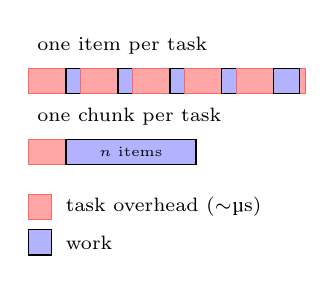
\begin{tikzpicture}[x=0.3cm, y=1cm, font=\scriptsize,
					ov/.style={tl, fill=red!35, draw=red!60},
					wk/.style={tl, fill=blue!30},
				]
				\node[anchor=west] at (0,0.45) {one item per task};
				\foreach \k in {0,...,4} {
						\tlseg{ov}{2.2*\k}{1.6}{0}{}
						\tlseg{wk}{2.2*\k+1.6}{0.6}{0}{}
					}
				\node[anchor=west] at (0,-0.45) {one chunk per task};
				\tlseg{ov}{0}{1.6}{-0.9}{}
				\tlseg{wk}{1.6}{3}{-0.9}{\(n\) items}
				% legend
				\node[ov, minimum width=0.3cm] at (0,-1.6) {}; \node[anchor=west] at (1.2,-1.6) {task overhead (\(\sim\)\textmu s)};
				\node[wk, minimum width=0.3cm] at (0,-2.05) {}; \node[anchor=west] at (1.2,-2.05) {work};
			\end{tikzpicture}
		\end{column}
	\end{columns}

	\vfill
	\begin{itemize}
		\item Every task pays a fixed cost: create, schedule, wait (\(\sim\)\textmu s)
		\item A chunk of \(n\) items pays it \alert{once}: keep \(n \times\) (cost per item) \(\gg\) task cost
		\item Too few chunks: one slow chunk leaves threads idle \(\Rightarrow\) \alert{balance} (next)
	\end{itemize}

	\begin{tcolorbox}[talk=red!70!black, boxsep=1pt, top=1pt, bottom=1pt, fontupper=\small\raggedright]
		\faExclamationTriangle\ Cost per item: usually \alert{unknown}, and varies from run to run\\
		\(\Rightarrow\) hard to predict: \alert{measure}, and keep a few chunks per thread
	\end{tcolorbox}

	\livedemo{granularity.jl}
\end{frame}

% ---------------------------------------------------------------------------
\begin{frame}[fragile]
	\frametitle{\texttt{@threads}: a convenience macro}
	\begin{columns}[c]
		\begin{column}{0.45\textwidth}
			\begin{minted}{julia}
@threads for i in 1:N
    ys[i] = f(xs[i])
end
			\end{minted}
		\end{column}
		\begin{column}{0.53\textwidth}
			\(=\) one task per chunk, then \alert{wait} for all: the code of the previous slide
		\end{column}
	\end{columns}

	\vfill
	\textbf{Schedules}: \texttt{@threads :greedy for i in \ldots}

	\smallskip
	\small
	\renewcommand{\arraystretch}{1.3}
	\begin{tabular}{@{}l>{\raggedright\arraybackslash}p{9.2cm}@{}}
		\texttt{:dynamic} & default: \(\sim\)\texttt{nthreads()} contiguous chunks \\
		\texttt{:greedy}  & \texttt{nthreads()} tasks, each takes the \alert{next item} when free: uneven work, any iterator \\
		\texttt{:static}  & one task \alert{pinned} per thread: \texttt{threadid()} constant; cannot be nested, discouraged \\
	\end{tabular}

	\vfill
	\normalsize
	\begin{tcolorbox}[talk, boxsep=1pt, top=1pt, bottom=1pt, fontupper=\small\raggedright]
		\faLightbulb\ \textbf{Use it for independent loops.} To combine results (e.g.\ a sum):\\
		protect the shared state (lock, atomic) \hfill \textit{later}
	\end{tcolorbox}

	\livedemo{threads_loop.jl}
\end{frame}

% ---------------------------------------------------------------------------
\begin{frame}[fragile]
	\frametitle{Reusing memory: buffers}
	\textbf{Many systems}: \(N = 100\) solves of size \(1000\), single thread

	\medskip
	\begin{columns}[T]
		\begin{column}{0.48\textwidth}
			\textbf{Allocate} every time:
			\begin{minted}{julia}
for i in 1:N
    F = lu(As[i])
    xs[i] = F \ bs[i]
end
			\end{minted}
		\end{column}
		\begin{column}{0.48\textwidth}
			\textbf{Buffer}: allocate once, overwrite:
			\begin{minted}{julia}
F = lu(As[1])
for i in 1:N
    lu!(F, As[i])  # writes into F
    xs[i] = F \ bs[i]
end
			\end{minted}
		\end{column}
	\end{columns}

	\medskip
	\centering
	Memory: \alert{766 MiB} allocated in total \quad vs.\ \quad \alert{8 MiB}, one \texttt{F} reused

	\vfill
	\punchline{With threads: one buffer per \alert{what}?}

	\livedemoopt{buffers.jl}
\end{frame}

% ---------------------------------------------------------------------------
\begin{frame}[fragile]
	\frametitle{Tempting: one buffer per thread}
	\begin{minted}{julia}
Fs = [lu(As[1]) for _ in 1:maxthreadid()]  # one per thread id
@threads for i in 1:N
    F = Fs[threadid()]
    lu!(F, As[i])
    xs[i] = F \ bs[i]
end
	\end{minted}

	\begin{itemize}
		\item Runs, right answer\ldots\ and \alert{wrong}
	\end{itemize}

	\centering
	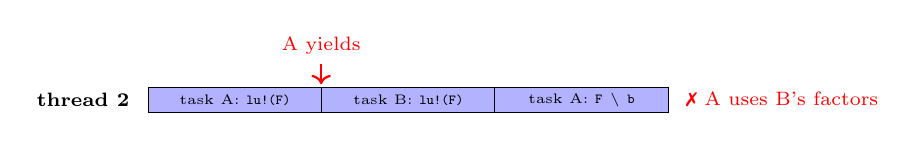
\begin{tikzpicture}[x=0.55cm, y=1cm, font=\scriptsize]
		\node[anchor=east] at (-0.2,0) {\textbf{thread 2}};
		\tlseg{running}{0}{4}{0}{task A: \texttt{lu!(F)}}
		\tlseg{running}{4}{4}{0}{task B: \texttt{lu!(F)}}
		\tlseg{running}{8}{4}{0}{task A: \texttt{F \textbackslash{} b}}
		\draw[->, thick, red] (4,0.45) node[above] {A yields} -- (4,0.2);
		\node[text=red, anchor=west] at (12.2,0) {\xmark\ A uses B's factors};
	\end{tikzpicture}

	\raggedright
	\begin{itemize}
		\item At a \alert{yield}, a task may \alert{migrate}, or another task may take its thread
		\item No yield in \texttt{lu!} today \(\Rightarrow\) correct \alert{by luck}, until it is not
	\end{itemize}

	\vfill
	\punchline{You write \alert{tasks}, not threads}

	\livedemoopt{threadid.jl}
\end{frame}

% ---------------------------------------------------------------------------
\begin{frame}[fragile]
	\frametitle{Buffers belong to tasks}
	\begin{columns}[T]
		\begin{column}{0.5\textwidth}
			\textbf{By hand}: one buffer per chunk task
			\begin{minted}{julia}
n = cld(N, nthreads())  # chunk size
@sync for idxs in partition(1:N, n)
    @spawn begin
        F = lu(As[1])  # buffer
        for i in idxs
            lu!(F, As[i])
            xs[i] = F \ bs[i]
        end
    end
end
			\end{minted}
		\end{column}
		\begin{column}{0.48\textwidth}
			\textbf{With \texttt{@threads}}: \texttt{OncePerTask}
			\begin{minted}{julia}
F0 = lu(As[1])
buf = OncePerTask(() -> copy(F0))
@threads for i in 1:N
    F = buf()  # buffer
    lu!(F, As[i])
    xs[i] = F \ bs[i]
end
			\end{minted}
			\textcolor{gray}{\small Julia \(\geq\) 1.12}
		\end{column}
	\end{columns}

	\vfill
	\begin{itemize}
		\item Buffers \(=\) tasks \(=\) chunks \(\approx\) threads, not iterations: \(20\times\) less memory
		\item \texttt{buf()}: runs the initializer \alert{once per task}, then returns the same buffer
		\item Each loop: new tasks \(\Rightarrow\) new buffers
	\end{itemize}

	\livedemo{buffers_threads.jl}
\end{frame}

% ---------------------------------------------------------------------------
\begin{frame}[fragile]
	\frametitle{Load balancing: how many chunks?}
	\textbf{Unequal work}: sizes \(200 \to 1600\), cost \(\propto m^3\): the last items dominate

	\medskip
	\centering
	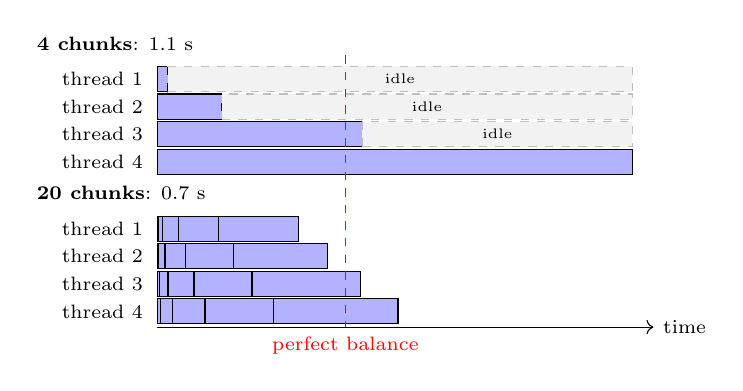
\begin{tikzpicture}[x=0.55cm, y=1cm, font=\scriptsize,
			idle/.style={tl, fill=gray!10, draw=gray!50, dashed},
		]
		% 4 chunks: one per thread, contiguous
		\node[anchor=west] at (-3.0,0.45) {\textbf{4 chunks}: 1.1 s};
		\foreach \th/\w in {0/0.23, 1/1.48, 2/4.73, 3/10.96} {
				\node[anchor=east] at (-0.1,-0.35*\th) {thread \the\numexpr\th+1};
				\tlseg{running}{0}{\w}{-0.35*\th}{}
				\pgfmathsetmacro{\r}{10.96-\w}
				\ifdim\r pt>0.01pt \tlseg{idle}{\w}{\r}{-0.35*\th}{idle} \fi
			}
		% 20 chunks: a free thread takes the next chunk
		\begin{scope}[yshift=-1.9cm]
			\node[anchor=west] at (-3.0,0.45) {\textbf{20 chunks}: 0.7 s};
			\foreach \th in {0,...,3} {\node[anchor=east] at (-0.1,-0.35*\th) {thread \the\numexpr\th+1};}
			\foreach \th/\t/\w in {0/0.00/0.01, 1/0.00/0.02, 2/0.00/0.04, 3/0.00/0.06, 0/0.01/0.10, 1/0.02/0.15, 2/0.04/0.21, 3/0.06/0.28, 0/0.11/0.37, 1/0.17/0.48, 2/0.24/0.60, 3/0.34/0.75, 0/0.48/0.92, 1/0.64/1.12, 2/0.85/1.33, 3/1.10/1.58, 0/1.40/1.86, 1/1.76/2.16, 2/2.18/2.50, 3/2.68/2.87} {
					\tlseg{running}{\t}{\w}{-0.35*\th}{}
				}
		\end{scope}
		% perfect balance: total work / 4
		\draw[dashed, red] (4.35,0.3) -- (4.35,-3.15) node[below, text=red] {perfect balance};
		\draw[->] (0,-3.15) -- (11.46,-3.15) node[right] {time};
	\end{tikzpicture}

	\vfill
	\raggedright
	\begin{itemize}
		\item 4 chunks: the last one holds \(63\%\) of the work
		\item More chunks: a free thread takes the next one \(\Rightarrow\) \alert{balance}
		\item Cost: more tasks, more buffers
	\end{itemize}

	\livedemoopt{load_balance.jl}
\end{frame}

% ---------------------------------------------------------------------------
\begin{frame}[fragile]
	\frametitle{Borrowing buffers: a pool}
	\begin{columns}[T]
		\begin{column}{0.56\textwidth}
			\begin{minted}{julia}
F0 = lu(As[1])
pool = Channel{typeof(F0)}(nthreads())
for _ in 1:nthreads()
    put!(pool, copy(F0))  # cheap
end
@threads for i in 1:N
    F = take!(pool)  # wait if empty
    lu!(F, As[i])
    xs[i] = F \ bs[i]
    put!(pool, F)    # give it back
end
			\end{minted}
		\end{column}
		\begin{column}{0.42\textwidth}
			\centering
			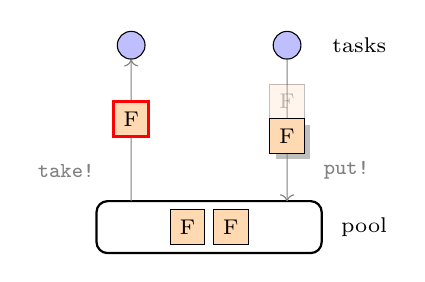
\begin{tikzpicture}[scale=1.1, transform shape,
					font=\scriptsize,
					task/.style={draw, circle, fill=blue!25, minimum size=0.32cm, inner sep=0pt},
					buf/.style={draw, fill=orange!30, minimum size=0.4cm, inner sep=0pt},
				]
				% two running tasks: one takes a buffer, one gives its buffer back
				\node[task] (ta) at (0.1,2.6) {};
				\node[task] (tb) at (1.9,2.6) {};
				\node[anchor=west] at (2.3,2.6) {tasks};
				% the pool: buffers not in use (4 in total)
				\node[draw, thick, rounded corners, minimum width=2.6cm, minimum height=0.6cm] (pool) at (1.0,0.5) {};
				\node[buf] at (0.75,0.5) {F};
				\node[buf] at (1.25,0.5) {F};
				\node[anchor=west] at (2.4,0.5) {pool};
				% take!: highlighted buffer on its way up
				\draw[->, gray] (0.1,0.8) -- (ta.south);
				\node[anchor=east, text=gray] at (-0.2,1.15) {\texttt{take!}};
				\node[buf, draw=red, very thick] at (0.1,1.75) {F};
				% put!: buffer on its way down, with a trail
				\draw[->, gray] (tb.south) -- (1.9,0.8);
				\node[anchor=west, text=gray] at (2.2,1.15) {\texttt{put!}};
				\node[buf, opacity=0.25] at (1.9,1.95) {F};
				\node[buf, drop shadow] at (1.9,1.55) {F};
			\end{tikzpicture}

		\end{column}
	\end{columns}

	\vfill
	\begin{itemize}
		\item Tasks \alert{borrow} a buffer, do not own one: buffers \alert{outlive} the loop
		\item Any schedule, any number of tasks: \alert{bounded} number of buffers
		\item Setup runs on \alert{one thread}: one \texttt{lu}, then cheap copies
	\end{itemize}

	\livedemo{buffers_threads.jl}
\end{frame}

% ---------------------------------------------------------------------------
\begin{frame}[fragile]
	\frametitle{Accumulating: sum of log-determinants}
	\begin{columns}[T]
		\begin{column}{0.52\textwidth}
			\begin{minted}{julia}
ld = 0.0
@threads for i in 1:N
    F = lu(As[i])
    xs[i] = F \ bs[i]
    ld += logdet(F)  # race!
end
			\end{minted}

			\medskip
			\small
			\begin{tabular}{ll}
				\texttt{-t 1} & exact \cmark                                \\
				\texttt{-t 4} & 3--8\,\% too small, varies \xmark \\
			\end{tabular}
		\end{column}
		\begin{column}{0.46\textwidth}
			\centering
			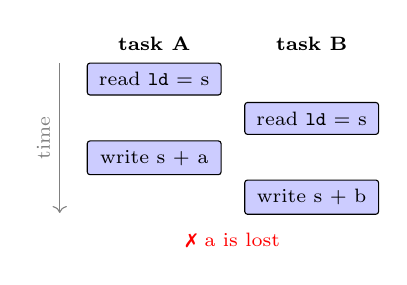
\begin{tikzpicture}[x=1cm, y=0.5cm, font=\scriptsize,
					op/.style={draw, fill=blue!20, rounded corners=1pt, minimum width=1.7cm, minimum height=0.38cm}]
				\node at (0,0.9) {\textbf{task A}};
				\node at (2,0.9) {\textbf{task B}};
				\node[op] at (0,0) {read \texttt{ld} = s};
				\node[op] at (2,-1) {read \texttt{ld} = s};
				\node[op] at (0,-2) {write s + a};
				\node[op] at (2,-3) {write s + b};
				\draw[->, gray] (-1.2,0.4) -- (-1.2,-3.4) node[midway, left, rotate=90, anchor=south] {time};
				\node[text=red] at (1,-4.1) {\xmark\ a is lost};
			\end{tikzpicture}
		\end{column}
	\end{columns}

	\vfill
	\begin{itemize}
		\item \texttt{+=} is \alert{read, add, write}: tasks interleave \(\Rightarrow\) lost updates
		\item Wrong \alert{silently}: no error, plausible number
	\end{itemize}

	\livedemo{accumulate.jl}
\end{frame}

% ---------------------------------------------------------------------------
\begin{frame}[fragile]
	\frametitle{Fixing the race}
	Combine the \texttt{d = logdet(F)} of each iteration:

	\medskip
	\begin{columns}[c]
		\begin{column}{0.3\textwidth}
			\textbf{Lock}\\
			{\footnotesize\textcolor{gray}{one task at a time; others queue}}
		\end{column}
		\begin{column}{0.68\textwidth}
			\begin{minted}{julia}
ld = Lockable(Ref(0.0))
@lock ld ld[][] += d  # in the loop
			\end{minted}
		\end{column}
	\end{columns}
	\medskip
	\begin{columns}[c]
		\begin{column}{0.3\textwidth}
			\textbf{Atomic}\\
			{\footnotesize\textcolor{gray}{indivisible update; primitive types only}}
		\end{column}
		\begin{column}{0.68\textwidth}
			\begin{minted}{julia}
ld = Atomic{Float64}(0.0)
atomic_add!(ld, d)    # in the loop
			\end{minted}
		\end{column}
	\end{columns}
	\medskip
	\begin{columns}[c]
		\begin{column}{0.3\textwidth}
			\textbf{No sharing}\\
			{\footnotesize\textcolor{gray}{each task returns a partial sum; own tasks}}
		\end{column}
		\begin{column}{0.68\textwidth}
			\begin{minted}{julia}
ts = map(chunks) do idxs
    @spawn sum(i -> logdet(lu(As[i])), idxs)
end
ld = sum(fetch.(ts))
			\end{minted}
		\end{column}
	\end{columns}

	\vfill
	\begin{itemize}
		\item Lock, atomic: order of additions varies \(\Rightarrow\) \alert{last digits} vary
	\end{itemize}

	\livedemo{accumulate.jl}
\end{frame}

% ---------------------------------------------------------------------------
\begin{frame}[fragile]
	\frametitle{Fixing the race: a lock}
	\begin{columns}[T]
		\begin{column}{0.56\textwidth}
			\begin{minted}{julia}
ld = Lockable(Ref(0.0))
@threads for i in 1:N
    F = lu(As[i])
    xs[i] = F \ bs[i]
    d = logdet(F)  # outside the lock
    @lock ld ld[][] += d
end
@lock ld ld[][]
			\end{minted}
		\end{column}
		\begin{column}{0.42\textwidth}
			\texttt{@lock l expr} is sugar for:
			\begin{minted}{julia}
lock(l)
try
    expr
finally
    unlock(l)
end
			\end{minted}
		\end{column}
	\end{columns}

	\vfill
	\begin{itemize}
		\item \texttt{lock}: one task at a time in the \alert{critical section}; others wait
		\item \texttt{Lockable}: value + lock, value only reached \alert{under} the lock
		\item Keep the critical section short: compute outside, update inside
		\item Correct, same speed: \(0.49\,\text{s}\) (\texttt{-t 4})
	\end{itemize}

	\livedemo{accumulate.jl}
\end{frame}

\subsection{Dependent tasks}

% ---------------------------------------------------------------------------
\begin{frame}
	\frametitle{Example: \(2\times 2\) block LU}
	\textbf{One big matrix} instead of many: tiles \(\Rightarrow\) tasks \alert{depend} on each other
	\[
		\begin{pmatrix} A_{11} & A_{12} \\ A_{21} & A_{22} \end{pmatrix}
		=
		\begin{pmatrix} L_{11} & \\ L_{21} & L_{22} \end{pmatrix}
		\begin{pmatrix} U_{11} & U_{12} \\ & U_{22} \end{pmatrix}
	\]

	\vfill
	\begin{columns}[c]
		\column{0.55\textwidth}
		\small
		\renewcommand{\arraystretch}{1.3}
		\begin{tabular}{c l l}
			\textbf{1} & \(A_{11} = L_{11} U_{11}\)                    & \texttt{lu!}             \\
			\textbf{2} & \(U_{12} = L_{11}^{-1} A_{12}\)               & \texttt{ldiv!}           \\
			\textbf{3} & \(L_{21} = A_{21} U_{11}^{-1}\)               & \texttt{rdiv!}           \\
			\textbf{4} & \(L_{22} U_{22} = A_{22} - L_{21} U_{12}\)    & \texttt{mul!}, \texttt{lu!} \\
		\end{tabular}

		\column{0.2\textwidth}
		\centering
		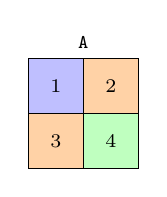
\begin{tikzpicture}[font=\scriptsize, scale=0.7]
			\draw[fill=blue!25] (0,1) rectangle (1,2) node[midway] {1};
			\draw[fill=orange!35] (1,1) rectangle (2,2) node[midway] {2};
			\draw[fill=orange!35] (0,0) rectangle (1,1) node[midway] {3};
			\draw[fill=green!25] (1,0) rectangle (2,1) node[midway] {4};
			\node[above] at (1,2) {\texttt{A}};
		\end{tikzpicture}

		\column{0.2\textwidth}
		\centering
		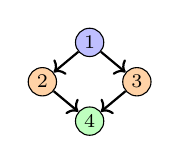
\begin{tikzpicture}[font=\scriptsize, x=0.6cm, y=0.5cm,
				nd/.style={draw, circle, inner sep=1.5pt}]
			\node[nd, fill=blue!25] (1) at (0,0) {1};
			\node[nd, fill=orange!35] (2) at (-1,-1) {2};
			\node[nd, fill=orange!35] (3) at (1,-1) {3};
			\node[nd, fill=green!25] (4) at (0,-2) {4};
			\draw[->, thick] (1) -- (2);
			\draw[->, thick] (1) -- (3);
			\draw[->, thick] (2) -- (4);
			\draw[->, thick] (3) -- (4);
		\end{tikzpicture}
	\end{columns}

	\vfill
	\begin{itemize}
		\item In place: \(L\) and \(U\) overwrite \(A\), tile by tile
		\item Order matters: 2 and 3 need 1; 4 needs 2 and 3
	\end{itemize}

	\begin{tcolorbox}[talk=red!70!black, boxsep=1pt, top=1pt, bottom=1pt, fontupper=\small\raggedright]
		\faExclamationTriangle\ \alert{Dependent} tasks: in general \alert{much harder} than independent iterations\\
		\(\Rightarrow\) who waits for whom, and when?
	\end{tcolorbox}
\end{frame}

% ---------------------------------------------------------------------------
\begin{frame}[fragile]
	\frametitle{Coordination is your job}
	\textbf{One task per step}, no coordination:
	\begin{minted}{julia}
t1 = @spawn lu!(A11, NoPivot())
t2 = @spawn ldiv!(UnitLowerTriangular(A11), A12)  # needs t1!
t3 = @spawn rdiv!(A21, UpperTriangular(A11))      # needs t1!
t4 = @spawn begin                                 # needs t2, t3!
    mul!(A22, A21, A12, -1, 1)
    lu!(A22, NoPivot())
end
	\end{minted}

	\vfill
	\centering
	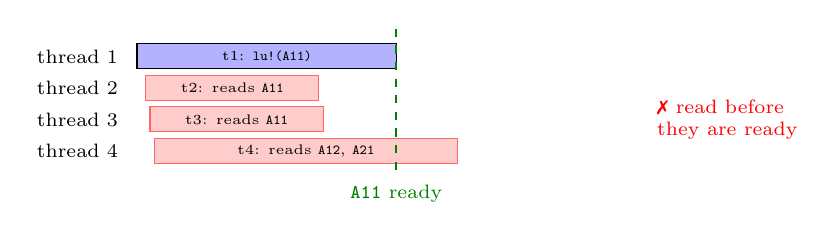
\begin{tikzpicture}[x=0.55cm, y=1cm, font=\scriptsize,
			bad/.style={tl, fill=red!20, draw=red!60},
		]
		\node[anchor=east] at (-0.2,0) {thread 1};
		\tlseg{running}{0}{6}{0}{t1: \texttt{lu!(A11)}}
		\node[anchor=east] at (-0.2,-0.4) {thread 2};
		\tlseg{bad}{0.2}{4}{-0.4}{t2: reads \texttt{A11}}
		\node[anchor=east] at (-0.2,-0.8) {thread 3};
		\tlseg{bad}{0.3}{4}{-0.8}{t3: reads \texttt{A11}}
		\node[anchor=east] at (-0.2,-1.2) {thread 4};
		\tlseg{bad}{0.4}{7}{-1.2}{t4: reads \texttt{A12}, \texttt{A21}}
		\draw[dashed, thick, green!50!black] (6,0.35) -- (6,-1.5) node[below] {\texttt{A11} ready};
		\node[text=red, anchor=west, align=left] at (11.8,-0.8) {\xmark\ read \alert{before}\\ they are ready};
	\end{tikzpicture}

	\vfill
	\raggedright
	\begin{itemize}
		\item \texttt{-t 1}: error \(5\times10^{-16}\), correct \alert{by luck} (tasks run in spawn order)
		\item \texttt{-t 4}: error \(10^{7}\ldots10^{11}\), changes every run: \alert{silent}, \alert{nondeterministic}
	\end{itemize}

	\livedemo{lu_nowait.jl}
\end{frame}

% ---------------------------------------------------------------------------
\begin{frame}[fragile, label=yield-points]
	\frametitle{Coordinating tasks}
	\begin{itemize}
		\item \textbf{Protect shared data:} \texttt{lock}, atomics \hfill\textcolor{gray}{\cmark\ seen}
		\item \textbf{Communicate:} \texttt{Channel} \hfill\textcolor{gray}{\cmark\ seen}
		\item \textbf{Order:} \texttt{wait}, \texttt{fetch} \hfill\alert{now}
	\end{itemize}

	\vfill
	\punchline{\texttt{wait(x)}: suspend until \texttt{x} says go}
	\vspace{-0.6em}
	\centering{\small\textcolor{gray}{every blocking call is a \texttt{wait} underneath: \texttt{lock}, \texttt{take!}, \texttt{fetch}, \texttt{@sync}, \texttt{sleep}}}

	\vfill
	\begin{columns}[c]
		\column{0.45\textwidth}
		\centering\small
		\renewcommand{\arraystretch}{1.2}
		\begin{tabular}{l l}
			\textbf{\texttt{x}} & \textbf{wait until\ldots} \\
			\hline
			\texttt{Task}       & it is done                \\
			\texttt{Condition}  & \texttt{notify(x)}        \\
			\texttt{Event}      & \texttt{notify(x)}        \\
			\texttt{Channel}    & data is available         \\
			\texttt{Timer}      & it fires                  \\
		\end{tabular}

		\column{0.52\textwidth}
		\begin{onlyenv}<1>
			\texttt{fetch} \(\approx\) \texttt{wait} + read result
			\begin{minted}{julia}
function fetch(t::Task)
    wait(t)
    return t.result
end
			\end{minted}
		\end{onlyenv}
		\begin{onlyenv}<2>
			\texttt{sleep} \(\approx\) \texttt{wait} on a timer
			\begin{minted}{julia}
function sleep(s)
    wait(Timer(s))
end
			\end{minted}
		\end{onlyenv}
		\textcolor{gray}{\scriptsize simplified from Julia's \texttt{Base}}

		\medskip
	\end{columns}
\end{frame}

% ---------------------------------------------------------------------------
\begin{frame}[fragile]
	\frametitle{Dependencies by hand: \texttt{wait}}
	Each task \alert{waits} for its inputs:
	\begin{minted}[fontsize=\scriptsize]{julia}
t1 = @spawn lu!(A11, NoPivot())
t2 = @spawn (wait(t1); ldiv!(UnitLowerTriangular(A11), A12))
t3 = @spawn (wait(t1); rdiv!(A21, UpperTriangular(A11)))
t4 = @spawn begin
    wait(t2); wait(t3)
    mul!(A22, A21, A12, -1, 1)
    lu!(A22, NoPivot())
end
wait(t4)
	\end{minted}

	\vfill
	\centering
	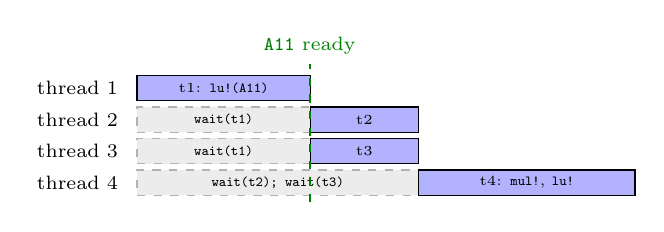
\begin{tikzpicture}[x=0.55cm, y=1cm, font=\scriptsize]
		\node[anchor=east] at (-0.2,0) {thread 1};
		\tlseg{running}{0}{4}{0}{t1: \texttt{lu!(A11)}}
		\node[anchor=east] at (-0.2,-0.4) {thread 2};
		\tlseg{blocked}{0}{4}{-0.4}{\texttt{wait(t1)}}
		\tlseg{running}{4}{2.5}{-0.4}{t2}
		\node[anchor=east] at (-0.2,-0.8) {thread 3};
		\tlseg{blocked}{0}{4}{-0.8}{\texttt{wait(t1)}}
		\tlseg{running}{4}{2.5}{-0.8}{t3}
		\node[anchor=east] at (-0.2,-1.2) {thread 4};
		\tlseg{blocked}{0}{6.5}{-1.2}{\texttt{wait(t2); wait(t3)}}
		\tlseg{running}{6.5}{5}{-1.2}{t4: \texttt{mul!}, \texttt{lu!}}
		\draw[dashed, thick, green!50!black] (4,-1.45) -- (4,0.3) node[above] {\texttt{A11} ready};
	\end{tikzpicture}

	\vfill
	\raggedright
	\begin{itemize}
		\item Correct on any number of threads; one \texttt{wait} per \alert{edge} of the graph
		\item Only 2 \(\parallel\) 3; the two \texttt{lu!} run in sequence: \(2.8\,\text{s} \to 2.5\,\text{s}\) \(\Rightarrow\) need \alert{more tiles}
	\end{itemize}

	\livedemo{lu_2x2.jl}
\end{frame}

% ---------------------------------------------------------------------------
\begin{frame}
	\frametitle{More tiles, more dependencies}
	\(3\times3\) tiles: one node \(=\) one kernel on one tile, one arrow \(=\) one \texttt{wait}

	\medskip
	\centering
	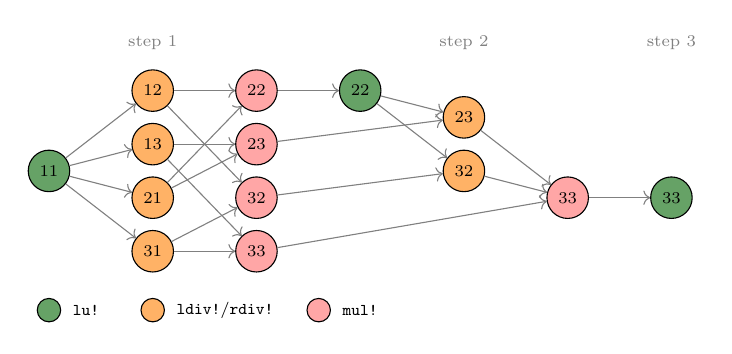
\begin{tikzpicture}[lugraph, c/.style={e}, scale=0.85, every node/.style={transform shape}]
		\lugraph
		\node[text=gray] at (1,2.4) {step 1};
		\node[text=gray] at (4,2.4) {step 2};
		\node[text=gray] at (6,2.4) {step 3};
		\node[lu, minimum size=0.35cm] at (0,-2.6) {}; \node[anchor=west] at (0.15,-2.6) {\texttt{lu!}};
		\node[pan, minimum size=0.35cm] at (1,-2.6) {}; \node[anchor=west] at (1.15,-2.6) {\texttt{ldiv!}/\texttt{rdiv!}};
		\node[up, minimum size=0.35cm] at (2.6,-2.6) {}; \node[anchor=west] at (2.75,-2.6) {\texttt{mul!}};
	\end{tikzpicture}

	\vfill
	\raggedright
	\begin{itemize}
		\item \(3\times3\): 14 tasks, 21 edges; \(n\times n\): \(\sim n^3/3\) tasks
		\item By hand: track \alert{who last wrote} each tile: error-prone
		\item How to enforce them? Two ways by hand: \alert{phases}, or \alert{last writers}
	\end{itemize}
\end{frame}

% ---------------------------------------------------------------------------
\begin{frame}[fragile]
	\frametitle{Fork-join: dependencies as phases}
	\begin{minted}[fontsize=\scriptsize]{julia}
for k in 1:n
    lu!(T[k,k], NoPivot())
    @sync begin  # panels
        for j in k+1:n; @spawn ldiv!(...); end
        for i in k+1:n; @spawn rdiv!(...); end
    end
    @sync for j in k+1:n, i in k+1:n  # updates
        @spawn mul!(T[i,j], T[i,k], T[k,j], -1, 1)
    end
end
	\end{minted}

	\centering
	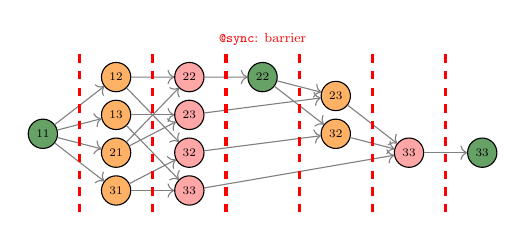
\begin{tikzpicture}[lugraph, scale=0.6, every node/.style={transform shape}, c/.style={e}]
		\lugraph
		\foreach \x in {0.5,1.5,...,5.5} {\draw[very thick, dashed, red] (\x,2.1) -- (\x,-2.1);}
		\node[text=red, font=\footnotesize] at (3,2.5) {\texttt{@sync}: barrier};
	\end{tikzpicture}

	\raggedright
	\begin{itemize}
		\item Parallel \alert{within} a phase; wait for \alert{all} of it before the next
		\item Simple, often good (\(0.86 \to 0.18\) s); but barriers idle threads
	\end{itemize}

	\livedemo{lu_tiled.jl}
\end{frame}

% ---------------------------------------------------------------------------
\begin{frame}
	\frametitle{Tasks by hand: a last-writer table}
	\textbf{No barriers.} Keep \texttt{W[i,j]}: the \alert{last task that wrote} tile \((i,j)\)

	\medskip
	\begin{tcolorbox}[talk, boxsep=1pt, top=1pt, bottom=1pt]
		Each new task: \textbf{1.} waits for the last writers of the tiles it \alert{uses};
		\textbf{2.} becomes the last writer of the tile it \alert{writes}
	\end{tcolorbox}

	\begin{columns}[c]
		\begin{column}{0.36\textwidth}
			\centering
			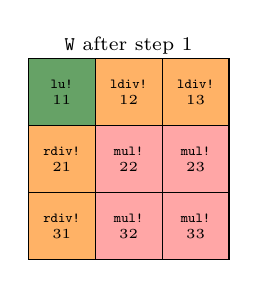
\begin{tikzpicture}[x=0.85cm, y=0.85cm, font=\tiny,
					cell/.style={draw, minimum size=0.85cm, inner sep=0pt, align=center}]
				\node[cell, fill=themegreen!60] at (1,-1) {\texttt{lu!}\\11};
				\foreach \j in {2,3} {\node[cell, fill=orange!60] at (\j,-1) {\texttt{ldiv!}\\1\j};}
				\foreach \i in {2,3} {\node[cell, fill=orange!60] at (1,-\i) {\texttt{rdiv!}\\\i1};}
				\foreach \i in {2,3} {\foreach \j in {2,3} {\node[cell, fill=red!35] at (\j,-\i) {\texttt{mul!}\\\i\j};}}
				\node[font=\scriptsize] at (2,-0.3) {\texttt{W} after step 1};
			\end{tikzpicture}
		\end{column}
		\begin{column}{0.62\textwidth}
			\small
			Step 2, in loop order:
			\begin{itemize}
				\item \texttt{lu!} of 22 waits for \texttt{W[2,2]} (\texttt{mul!} 22)\\
				      then \texttt{W[2,2]} \(=\) this task
				\item \texttt{ldiv!} of 23 waits for \texttt{W[2,2]}, \texttt{W[2,3]}
				\item \texttt{mul!} of 33 waits for \texttt{W[3,2]}, \texttt{W[2,3]}, \texttt{W[3,3]}
			\end{itemize}
		\end{column}
	\end{columns}

\end{frame}

% ---------------------------------------------------------------------------
\begin{frame}
	\frametitle{Tasks by hand: no barriers}
	\centering
	\begin{tikzpicture}[lugraph, scale=0.85, every node/.style={transform shape}, c/.style={e}]
		\lugraph
		\node[draw=structure, very thick, circle, minimum size=0.85cm] at (L2) {};
		\node[text=structure, font=\footnotesize, align=left, anchor=west] at (3.3,2.3)
			{\texttt{lu!} of 22 starts as soon as 22 is updated,\\ while 23, 32, 33 are still updating};
	\end{tikzpicture}

	\vfill
	\raggedright
	\begin{itemize}
		\item The waits \alert{are} the arrows, found while running the sequential loop
		\item A task starts when its inputs are ready: step \(k+1\) overlaps step \(k\)
		\item Fork-join waits for the \alert{whole} step instead
	\end{itemize}
\end{frame}

% ---------------------------------------------------------------------------
\begin{frame}[fragile]
	\frametitle{Tasks by hand: the code}
	\begin{columns}[T]
		\begin{column}{0.68\textwidth}
			\begin{minted}[fontsize=\scriptsize]{julia}
spawn_after(f, deps...) = @spawn (waitall(deps); f())
W = fill(@spawn(nothing), n, n)  # last writers
for k in 1:n
    W[k,k] = spawn_after(W[k,k]) do
        lu!(T[k,k], NoPivot())
    end
    for j in k+1:n  # panels
        W[k,j] = spawn_after(W[k,k], W[k,j]) do
            ldiv!(UnitLowerTriangular(T[k,k]), T[k,j])
        end
        W[j,k] = spawn_after(W[k,k], W[j,k]) do
            rdiv!(T[j,k], UpperTriangular(T[k,k]))
        end
    end
    for j in k+1:n, i in k+1:n  # updates
        W[i,j] = spawn_after(W[i,k], W[k,j], W[i,j]) do
            mul!(T[i,j], T[i,k], T[k,j], -1, 1)
        end
    end
end
waitall(W)
			\end{minted}
		\end{column}
		\begin{column}{0.3\textwidth}
			\footnotesize
			\begin{itemize}
				\item The sequential loop, each kernel wrapped in \texttt{spawn\_after}
				\item \texttt{deps}: evaluated \alert{now}, when the task is created
				\item 8 threads: fork-join 0.18 s, tasks \alert{0.16 s}
				\item Correct only because a tile that is read is \alert{never written again}
			\end{itemize}
		\end{column}
	\end{columns}

	\livedemo{lu_tiled.jl}
\end{frame}



\section{\DFT}

% --- ported from reference/2023-12-01_juliacon-local ---
\begin{frame}[fragile]
	\frametitle{Overview}
	\begin{itemize}
		\item \DFT{} is a Julia package dedicated to parallel programming on \textit{\textbf{multi-core shared memory CPUs}}
		\item \texttt{Task} dependencies inferred from \alert{data} annotations: \texttt{@R}, \texttt{@W}, \texttt{@RW}
		\item Simple API: the \texttt{@dspawn} macro
	\end{itemize}
	\hfill{\scriptsize\color{gray} In the spirit of StarPU, PaRSEC (not in ambition!)}

	\begin{columns}[T]
		\begin{column}{0.36\textwidth}
			\textbf{Sequential}
			\begin{minted}{julia}
function foo!(A, b)
  fill!(b, 0)
  view(b, 1:2) .+= 2
  view(b, 3:4) .+= 3
  A \ b
end
			\end{minted}
			\centering
			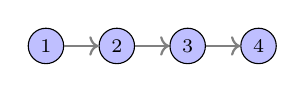
\begin{tikzpicture}[dag]
				\node[dnode] (1) at (0,0) {1};
				\node[dnode] (2) at (0.9,0) {2};
				\node[dnode] (3) at (1.8,0) {3};
				\node[dnode] (4) at (2.7,0) {4};
				\draw[dedge] (1) -- (2); \draw[dedge] (2) -- (3); \draw[dedge] (3) -- (4);
			\end{tikzpicture}
		\end{column}
		\begin{column}{0.62\textwidth}
			\textbf{With \DFT}: one task per line
			\begin{minted}{julia}
function foo!(A, b)
  @dspawn fill!(@W(b), 0)         # task 1
  @dspawn @RW(view(b, 1:2)) .+= 2 # task 2
  @dspawn @RW(view(b, 3:4)) .+= 3 # task 3
  @dspawn @R(A) \ @R(b)           # task 4
end
			\end{minted}
			\centering
			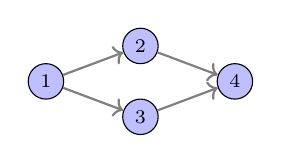
\begin{tikzpicture}[dag]
				\node[dnode] (1) at (0,0) {1};
				\node[dnode] (2) at (1.2,0.45) {2};
				\node[dnode] (3) at (1.2,-0.45) {3};
				\node[dnode] (4) at (2.4,0) {4};
				\draw[dedge] (1) -- (2); \draw[dedge] (1) -- (3); \draw[dedge] (2) -- (4); \draw[dedge] (3) -- (4);
			\end{tikzpicture}
		\end{column}
	\end{columns}
\end{frame}




\begin{frame}[fragile]
	\frametitle{Task based parallelism}
	\begin{itemize}
		\item A task is a unit of execution or a unit of work
		\item \texttt{Task} objects can be created using \texttt{@task}
		\item Once created, \texttt{Task} objects must be scheduled for execution
		\item Usually, \texttt{Task}s are created + scheduled using \texttt{@spawn}
		\item \alert{Responsibility of synchronizing tasks is left to the programmer}
	\end{itemize}

	\medskip
	\begin{columns}[T]
		\begin{column}{0.78\textwidth}
			\begin{overlayarea}{\linewidth}{3cm}
			\textbf{\only<1>{Sequential}\only<2>{Synchronizing tasks with return values}\only<3>{Synchronizing tasks with explicit waits}}
			\begin{onlyenv}<1>
				\begin{minted}{julia}
                      # task
b = zeros(4)          # 1: initialization
b[1:2] .+= 2          # 2: first half
b[3:4] .+= 3          # 3: second half
res = A \ b           # 4: entire vector
				\end{minted}
			\end{onlyenv}
			\begin{onlyenv}<2>
				\begin{minted}{julia}
t1 = @spawn zeros(4)                        # 1
t2 = @spawn (b = fetch(t1); b[1:2] .+ 2)    # 2
t3 = @spawn (b = fetch(t1); b[3:4] .+ 3)    # 3
t4 = @spawn A \ vcat(fetch(t2), fetch(t3))  # 4
fetch(t4) # get result
				\end{minted}
			\end{onlyenv}
			\begin{onlyenv}<3>
				\begin{minted}{julia}
b = Vector{Float64}(undef, 4)
t1 = @spawn fill!(b, 0)                     # 1
t2 = @spawn (wait(t1); view(b,1:2) .+= 2)   # 2
t3 = @spawn (wait(t1); view(b,3:4) .+= 3)   # 3
t4 = @spawn (wait(t2); wait(t3); A \ b)     # 4
fetch(t4) # get result
				\end{minted}
			\end{onlyenv}
			\end{overlayarea}
		\end{column}
		\begin{column}{0.2\textwidth}
			\centering
			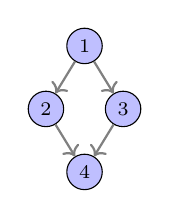
\begin{tikzpicture}[dag, x=0.7cm, y=0.8cm]
				\node[dnode] (1) at (0,0) {1};
				\node[dnode] (2) at (-0.7,-1) {2};
				\node[dnode] (3) at (0.7,-1) {3};
				\node[dnode] (4) at (0,-2) {4};
				\draw[dedge] (1) -- (2); \draw[dedge] (1) -- (3); \draw[dedge] (2) -- (4); \draw[dedge] (3) -- (4);
			\end{tikzpicture}
		\end{column}
	\end{columns}
\end{frame}


\begin{frame}[fragile]
	\frametitle{Motivation for \texttt{DataFlowTasks}}
	\begin{itemize}
		\item Reasoning about \texttt{Task} interdependencies can be challenging
		\item Especially for algorithms making constant re-use of data
		\item Sometimes, it is simpler to reason about how \texttt{Task}s depend on data than how \texttt{Task}s depend on each other
	\end{itemize}

	\medskip
	\textbf{Synchronizing tasks}
	\begin{minted}{julia}
b = rand(4)
t1 = @spawn fill!(b, 0)                    # W  access to b
t2 = @spawn (wait(t1); view(b,1:2) .+= 2)  # RW access to b[1:2]
t3 = @spawn (wait(t1); view(b,3:4) .+= 3)  # RW access to b[3:4]
t4 = @spawn (wait(t2); wait(t3); A \ b)    # R  access to A and b
fetch(t4)
	\end{minted}

	\vfill
	\onslide<2->{\punchline{Would like to declare only the \alert{task-to-data} dependencies}}
\end{frame}


\begin{frame}[fragile]

\frametitle{Basic idea}
\begin{enumerate}
    \item \textcolor<4->{lightgray}{Extract data dependency from user annotations}
    \item \textcolor<1-3,10->{lightgray}{Infer task dependency from data dependency}
    \item \textcolor<1-9>{lightgray}{Schedule tasks with inferred dependencies}
\end{enumerate}

\center
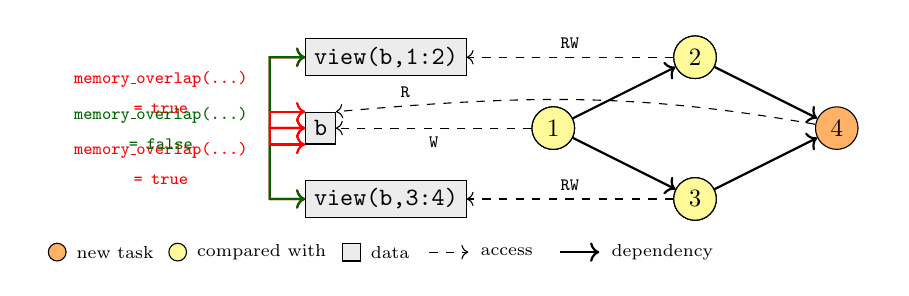
\begin{tikzpicture}[scale=0.9, every node/.style={transform shape}]
  % Tasks
  \node<2->[dnode, minimum size=0.6cm] (1) at (0,  0) {1};
  \node<2>[dnode, minimum size=0.6cm, fill=orange!60] at (0,  0) {1};
  \node<4,6,9>[dnode, minimum size=0.6cm, fill=yellow!40] at (0,  0) {1};
  
  \node<3->[dnode, minimum size=0.6cm] (2) at (2,  1) {2};
  \node<3-4>[dnode, minimum size=0.6cm, fill=orange!60] at (2,  1) {2};
  \node<5,8>[dnode, minimum size=0.6cm, fill=yellow!40] at (2,  1) {2};
  
  \node<5->[dnode, minimum size=0.6cm] (3) at (2, -1) {3};
  \node<5-6>[dnode, minimum size=0.6cm, fill=orange!60] at (2, -1) {3};
  \node<7>[dnode, minimum size=0.6cm, fill=yellow!40] at (2, -1) {3};

  \node<7->[dnode, minimum size=0.6cm, fill=orange!60] (4) at (4,  0) {4};
  
  % Data
  \node<1->[rectangle, draw, fill=gray!15, anchor=west] (A)  at (-3.5,  0) {\texttt{b}};
  \node<3->[rectangle, draw, fill=gray!15, anchor=west] (A1) at (-3.5,  1) {\texttt{view(b,1:2)}};
  \node<5->[rectangle, draw, fill=gray!15, anchor=west] (A2) at (-3.5, -1) {\texttt{view(b,3:4)}};
  
  % Task -> Data dependencies
  \draw<2->[->, dashed] (1) -- node[midway, below]{\scriptsize\ttfamily W} (A);
  \draw<3->[->, dashed] (2) -- node[midway, above]{\scriptsize\ttfamily RW} (A1) ;
  \draw<5->[->, dashed] (3) -- node[midway, above]{\scriptsize\ttfamily RW} (A2);
  \draw<7-> (4) edge[out=170, in=5, dashed, ->] node[pos=0.87, above]{\scriptsize\ttfamily R} (A.north east);
  
  % Task -> Task dependencies
  \draw<4->[->, thick] (1) -- (2);
  \draw<6->[->, thick] (1) -- (3);
  \draw<8->[->, thick] (2) -- (4);
  \draw<7->[->, thick] (3) -- (4);
  
  % Data <-> Data dependencies
  \draw<1-> (A.west)  ++(-0.5,0) node (Aw)  {};
  \draw<3-> (A1.west) ++(-0.5,0) node (A1w) {};
  \draw<5-> (A2.west) ++(-0.5,0) node (A2w) {};
  \draw<4,8>[<->, thick, red] (A.west)  -- (Aw.center)
  -- node[midway,left,text width=8em,align=center]{\scriptsize\ttfamily memory\_overlap(...) = true} (A1w.center) -- (A1.west);
  \draw<6,7>[<->, thick, red] (A.west)  -- (Aw.center)
  -- node[midway,left,text width=8em,align=center]{\scriptsize\ttfamily memory\_overlap(...) = true} (A2w.center) -- (A2.west);
  \draw<5>[<->, thick, themegreen] (A1.west) -- (A1w.center)
  -- node[midway,left,text width=8em,align=center]{\scriptsize\ttfamily memory\_overlap(...) = false} (A2w.center) -- (A2.west);
  \draw<9>[<->, thick, red] (A.south west) -- ++(-0.5,0) |- (A.north west);

  % Legend
  \begin{scope}[font=\scriptsize, lg/.style={dnode, minimum size=0.25cm}]
    \node[lg, fill=orange!60] at (-7.0,-1.75) {}; \node[anchor=west] at (-6.85,-1.75) {new task};
    \node[lg, fill=yellow!40] at (-5.3,-1.75) {}; \node[anchor=west] at (-5.15,-1.75) {compared with};
    \node[draw, fill=gray!15, minimum size=0.25cm, inner sep=0pt] at (-2.85,-1.75) {}; \node[anchor=west] at (-2.7,-1.75) {data};
    \draw[->, dashed] (-1.75,-1.75) -- (-1.2,-1.75); \node[anchor=west] at (-1.15,-1.75) {access};
    \draw[->, thick] (0.1,-1.75) -- (0.65,-1.75); \node[anchor=west] at (0.7,-1.75) {dependency};
  \end{scope}

  % Bounding box
  \node at (-7.3,-1.3) {};
  \node at (4.5,1.3) {};
\end{tikzpicture}

\begin{columns}[T]
  \column{0.42\textwidth}
\textbf{User-written code}
\begin{minted}[fontsize=\footnotesize,escapeinside=||,beameroverlays=true]{julia}
|\onslide<1->|b = rand(4)
|\onslide<2->|@dspawn fill!(@W(b),0)
|\onslide<3->|@dspawn @RW(view(b,1:2)) .+= 2
|\onslide<5->|@dspawn @RW(view(b,3:4)) .+= 3
|\onslide<7->|t4 = @dspawn A \ @R(b)
|\onslide<7->|fetch(t4)|\onslide<1->|
\end{minted}
  
  \column{0.50\textwidth}
\begin{onlyenv}<4-9>
\textbf{Behind the scenes: DAG}
\begin{minted}[fontsize=\footnotesize,escapeinside=||]{julia}
# Note the quadratic complexity!
for i in 1:N, j in i-1:-1:1
  # Detect conflict between i and j
  for di in data(i), dj in data(j)
    if memory_overlap(di, dj)
      add_edge(j, i)
\end{minted}
\end{onlyenv}
\begin{onlyenv}<10>
\textbf{Behind the scenes: scheduling}
\begin{minted}[fontsize=\footnotesize]{julia}
t4 = @spawn begin
  wait(t2); wait(t3)
  A \ b
end
\end{minted}
\end{onlyenv}
\end{columns}

% \alert{Note the quadratic complexity in the number of tasks!}

\end{frame}


% ---------------------------------------------------------------------------
\begin{frame}
	\frametitle{Under the hood: main types}
	\centering
	\begin{tikzpicture}[dag, x=1cm, y=1cm,
			box/.style={draw, rounded corners, thick},
			lbl/.style={font=\footnotesize\bfseries},
			ann/.style={font=\scriptsize, text=gray, align=left},
		]
		% TaskGraph
		\node[box, draw=structure, minimum width=9.6cm, minimum height=3.6cm] (tg) at (2.3,0) {};
		\node[lbl, text=structure, anchor=north west] at (tg.north west) {\texttt{TaskGraph}};
		% DAG
		\node[box, draw=gray, minimum width=4.6cm, minimum height=2.5cm] (dag) at (0.4,-0.2) {};
		\node[lbl, anchor=north west] at (dag.north west) {\texttt{DAG}};
		\node[dnode] (t1) at (-1.2,-0.2) {1};
		\node[dnode] (t2) at (0.2,0.35) {2};
		\node[dnode] (t3) at (0.2,-0.75) {3};
		\node[dnode] (t4) at (1.6,-0.2) {4};
		\draw[dedge] (t1) -- (t2); \draw[dedge] (t1) -- (t3); \draw[dedge] (t2) -- (t4); \draw[dedge] (t3) -- (t4);
		\node[ann, anchor=north] at (0.4,-1.05) {edges, lock, at most 50 tasks};
		% one DataFlowTask, zoomed
		\node[ann, anchor=west] (zoom) at (2.9,1.2) {node: a \texttt{DataFlowTask}\\\(=\) \texttt{Task} \(+\) data \(+\) access};
		\draw[gray, ->] (zoom.west) -- (t2);
		% cleaner
		\node[box, fill=orange!20, align=center, font=\scriptsize] (cl) at (5.6,-0.2) {cleaner task\\\texttt{:interactive}};
		\draw[->, thick] (t4.east) ++(0.25,0) -- node[above, font=\scriptsize] {finished} node[below, font=\scriptsize] {\texttt{put!}} (cl.west);
		\draw[->, thick, red!70!black] (cl.south) |- node[pos=0.75, below, font=\scriptsize] {\texttt{remove\_node!}} ($(dag.south east)+(0,0.3)$);
		% @dspawn
		\node[font=\scriptsize] (sp) at (-3.9,-0.2) {\texttt{@dspawn}};
		\draw[->, thick] (sp) -- node[above, font=\scriptsize] {\texttt{addnode!}} (dag.west);
	\end{tikzpicture}

	\vfill
	\raggedright
	\begin{itemize}
		\item \texttt{DataFlowTask}: a \texttt{Task} + the data it accesses, and how
		\item \texttt{DAG}: the dependencies between \texttt{DataFlowTask}s
		\item \texttt{TaskGraph}: a \texttt{DAG} + a task that removes finished tasks
	\end{itemize}

	\begin{tcolorbox}[talk, boxsep=1pt, top=1pt, bottom=1pt, fontupper=\small]
		\faLightbulb\ Built from the Part~1 primitives: \texttt{Task}, \texttt{wait}, \texttt{lock}, \texttt{Condition}, \texttt{Channel}
	\end{tcolorbox}
\end{frame}

% ---------------------------------------------------------------------------
\begin{frame}[fragile]
	\frametitle{\texttt{@dspawn}: what the macro does}
	\begin{itemize}
		\item Scan the expression for \texttt{@R}, \texttt{@W}, \texttt{@RW}; collect \texttt{data} and \texttt{access\_mode}
		\item Remove the annotations, wrap the code in a closure
		\item Call the \texttt{DataFlowTask} constructor, then schedule it
	\end{itemize}

	\vfill
	\textbf{User-written code}
	\begin{minted}{julia}
@dspawn foo!(@W(B), @R(A)) label = "foo!" priority = 1
	\end{minted}

	\bigskip
	\textbf{Macro expansion} (approx.)
	\begin{minted}{julia}
t = DataFlowTask(() -> foo!(B, A), (B, A), (WRITE, READ);
                 label = "foo!", priority = 1)  # 0: most urgent
t.task.sticky = false       # like @spawn
_spawn_set_thrpool(t.task, :default)  # else: parent's pool
schedule(t.task)
	\end{minted}

	\vfill
	\begin{itemize}
		\item Returns \texttt{t.task}, a plain \texttt{Task}: \texttt{wait}, \texttt{fetch} as usual
		\item \texttt{@dtask}: same, but not scheduled (\texttt{schedule} it yourself)
	\end{itemize}

\end{frame}

% ---------------------------------------------------------------------------
\begin{frame}[fragile]
	\frametitle{\texttt{DataFlowTask}: a task that waits for its dependencies}
	A \texttt{Task}, plus the data it accesses, how (access modes), and a priority

	\medskip
	\begin{columns}[T]
		\begin{column}{0.58\textwidth}
			\begin{onlyenv}<1>
				\begin{minted}[fontsize=\scriptsize, highlightlines={3-6}, highlightcolor=orange!25]{julia}
function DataFlowTask(f, data, mode, prio, tg)
    tj = new(data, mode)  # incomplete: no task yet
    deps = @lock tg.dag.lock begin
        addnode!(tg, tj)
        copy(inneighbors(tg.dag, tj))
    end
    tj.task = @task try
        waitall(deps; failfast = false)
        f()
    finally
        put!(tg.finished, tj)
    end
    tj.task.priority = prio
    return tj
end
				\end{minted}
			\end{onlyenv}
			\begin{onlyenv}<2>
				\begin{minted}[fontsize=\scriptsize, highlightlines={8}, highlightcolor=orange!25]{julia}
function DataFlowTask(f, data, mode, prio, tg)
    tj = new(data, mode)  # incomplete: no task yet
    deps = @lock tg.dag.lock begin
        addnode!(tg, tj)
        copy(inneighbors(tg.dag, tj))
    end
    tj.task = @task try
        waitall(deps; failfast = false)
        f()
    finally
        put!(tg.finished, tj)
    end
    tj.task.priority = prio
    return tj
end
				\end{minted}
			\end{onlyenv}
			\begin{onlyenv}<3>
				\begin{minted}[fontsize=\scriptsize, highlightlines={9}, highlightcolor=orange!25]{julia}
function DataFlowTask(f, data, mode, prio, tg)
    tj = new(data, mode)  # incomplete: no task yet
    deps = @lock tg.dag.lock begin
        addnode!(tg, tj)
        copy(inneighbors(tg.dag, tj))
    end
    tj.task = @task try
        waitall(deps; failfast = false)
        f()
    finally
        put!(tg.finished, tj)
    end
    tj.task.priority = prio
    return tj
end
				\end{minted}
			\end{onlyenv}
			\begin{onlyenv}<4>
				\begin{minted}[fontsize=\scriptsize, highlightlines={11}, highlightcolor=orange!25]{julia}
function DataFlowTask(f, data, mode, prio, tg)
    tj = new(data, mode)  # incomplete: no task yet
    deps = @lock tg.dag.lock begin
        addnode!(tg, tj)
        copy(inneighbors(tg.dag, tj))
    end
    tj.task = @task try
        waitall(deps; failfast = false)
        f()
    finally
        put!(tg.finished, tj)
    end
    tj.task.priority = prio
    return tj
end
				\end{minted}
			\end{onlyenv}
			\textcolor{gray}{\tiny simplified from \texttt{src/dataflowtask.jl}}
		\end{column}
		\begin{column}{0.4\textwidth}
			\centering
			\begin{tikzpicture}[dag, x=1.25cm, y=1.05cm, scale=1, every node/.append style={scale=1.15},
					done/.style={dnode, fill=gray!20, draw=gray!60, text=gray},
					run/.style={dnode, fill=blue!25},
					wt/.style={dnode, fill=white, draw=gray, dashed},
					new/.style={dnode, fill=orange!60},
				]
				% tasks 1..4 of the running example
				\node[done] (1) at (0,0) {1};
				\node<1-2>[run] (2) at (1,0.6) {2};
				\node<1-2>[run] (3) at (1,-0.6) {3};
				\node<3->[done] (2) at (1,0.6) {2};
				\node<3->[done] (3) at (1,-0.6) {3};
				\node<1>[new] (4) at (2,0) {4};
				\node<2>[wt] (4) at (2,0) {4};
				\node<3>[run] (4) at (2,0) {4};
				\node<4>[done] (4) at (2,0) {4};
				\draw[dedge, gray!50] (1) -- (2); \draw[dedge, gray!50] (1) -- (3);
				\draw<1-2>[dedge, very thick, orange] (2) -- (4);
				\draw<1-2>[dedge, very thick, orange] (3) -- (4);
				\draw<3->[dedge, gray!50] (2) -- (4); \draw<3->[dedge, gray!50] (3) -- (4);
				% lock around the DAG during insertion
				\node<1>[text=orange!80!black, font=\scriptsize] at (1,1.35) {\faLock\ \texttt{dag.lock}};
				% cleaner
				\node<4>[draw, rounded corners, fill=orange!20, font=\scriptsize] (cl) at (2,-1.6) {cleaner};
				\draw<4>[->, thick] (4) -- node[right, font=\scriptsize] {\texttt{put!}} (cl);
				% fixed bounding box: the picture does not move between steps
				\useasboundingbox (-0.4,-1.95) rectangle (2.6,1.6);
			\end{tikzpicture}

			\medskip
			\begin{overlayarea}{\linewidth}{1.6cm}
			\raggedright\small
			\only<1>{\textbf{1. Insert}, under the lock:\\ \texttt{deps} \(=\) \{2, 3\}, found from the \alert{data}}%
			\only<2>{\textbf{2. Wait} for \alert{all} \texttt{deps}, even if one fails}%
			\only<3>{\textbf{3. Run} the code: 2 and 3 are done}%
			\only<4>{\textbf{4. Report} in \texttt{finally}: always, even on error; the cleaner removes 4}
			\end{overlayarea}
		\end{column}
	\end{columns}
\end{frame}

% ---------------------------------------------------------------------------
\begin{frame}[fragile]
	\frametitle{\texttt{TaskGraph}: where the tasks live}
	\begin{columns}[T]
		\column{0.52\textwidth}
		\begin{minted}[fontsize=\scriptsize]{julia}
mutable struct TaskGraph
    dag::DAG{DataFlowTask}  # tasks + edges
    finished::FinishedChannel
    dag_cleaner::Task
end

# the cleaner, started with the TaskGraph
@spawn :interactive while true
    t = take!(tg.finished)
    t isa Stop && break
    remove_node!(tg, t)
end
		\end{minted}
		\textcolor{gray}{\tiny simplified from \texttt{src/taskgraph.jl}}

		\column{0.46\textwidth}
		\small
		\begin{itemize}
			\item Holds the \alert{unfinished} tasks and their edges
			\item \texttt{@dspawn} adds to the \alert{active} graph: the default one (50 tasks), or \texttt{with\_taskgraph}
			\item \texttt{wait(tg)}, \texttt{resize!(tg, n)}
			\item Finished task: \texttt{put!}; the cleaner (\alert{interactive} pool): \texttt{take!}, \texttt{remove\_node!}
		\end{itemize}
	\end{columns}

	\vfill
	\hfill\textcolor{gray}{\small Next: inside the \texttt{DAG} \(\to\)}
\end{frame}

% ---------------------------------------------------------------------------
\begin{frame}[fragile]
	\frametitle{\texttt{DAG}: a buffered, thread-safe graph}
	Nodes + edges, one \alert{lock}, two \texttt{Condition}s, \texttt{sz\_max} slots (default: 50)

	\medskip
	\begin{columns}[T]
		\begin{column}{0.56\textwidth}
			\begin{onlyenv}<1>
				\begin{minted}[fontsize=\scriptsize, highlightlines={6-7}, highlightcolor=orange!25]{julia}
function addnode!(dag, node)
    @lock dag begin
        while isfull(dag)  # sz_max nodes
            wait(dag.cond_push)
        end
        push!(dag.inoutlist, node => ...)
        update_edges!(dag, node)
    end
end
function remove_node!(dag, node)
    @lock dag begin
        pop!(dag.inoutlist, node)
        notify(dag.cond_push, all=false)
        isempty(dag) &&
            notify(dag.cond_empty)
    end
end
				\end{minted}
			\end{onlyenv}
			\begin{onlyenv}<2>
				\begin{minted}[fontsize=\scriptsize, highlightlines={3-5}, highlightcolor=orange!25]{julia}
function addnode!(dag, node)
    @lock dag begin
        while isfull(dag)  # sz_max nodes
            wait(dag.cond_push)
        end
        push!(dag.inoutlist, node => ...)
        update_edges!(dag, node)
    end
end
function remove_node!(dag, node)
    @lock dag begin
        pop!(dag.inoutlist, node)
        notify(dag.cond_push, all=false)
        isempty(dag) &&
            notify(dag.cond_empty)
    end
end
				\end{minted}
			\end{onlyenv}
			\begin{onlyenv}<3>
				\begin{minted}[fontsize=\scriptsize, highlightlines={12-13}, highlightcolor=orange!25]{julia}
function addnode!(dag, node)
    @lock dag begin
        while isfull(dag)  # sz_max nodes
            wait(dag.cond_push)
        end
        push!(dag.inoutlist, node => ...)
        update_edges!(dag, node)
    end
end
function remove_node!(dag, node)
    @lock dag begin
        pop!(dag.inoutlist, node)
        notify(dag.cond_push, all=false)
        isempty(dag) &&
            notify(dag.cond_empty)
    end
end
				\end{minted}
			\end{onlyenv}
			\begin{onlyenv}<4>
				\begin{minted}[fontsize=\scriptsize, highlightlines={14-15}, highlightcolor=orange!25]{julia}
function addnode!(dag, node)
    @lock dag begin
        while isfull(dag)  # sz_max nodes
            wait(dag.cond_push)
        end
        push!(dag.inoutlist, node => ...)
        update_edges!(dag, node)
    end
end
function remove_node!(dag, node)
    @lock dag begin
        pop!(dag.inoutlist, node)
        notify(dag.cond_push, all=false)
        isempty(dag) &&
            notify(dag.cond_empty)
    end
end
				\end{minted}
			\end{onlyenv}
			\textcolor{gray}{\tiny simplified from \texttt{src/dag.jl}}
		\end{column}
		\begin{column}{0.42\textwidth}
			\centering
			\begin{tikzpicture}[dag, x=0.75cm, y=0.8cm,
					slot/.style={draw, gray, rounded corners=2pt, minimum size=0.6cm},
					tk/.style={dnode, minimum size=0.45cm},
					new/.style={tk, fill=orange!60},
					wt/.style={tk, fill=white, draw=gray, dashed},
					gone/.style={tk, fill=gray!20, draw=gray!60, text=gray},
				]
				% the buffer: 4 slots (sz_max)
				\node[draw, rounded corners, minimum width=3.4cm, minimum height=0.9cm] (buf) at (1.5,0) {};
				\foreach \x in {0,...,3} {\node[slot] (s\x) at (\x,0) {};}
				% step 1: room, the new task enters
				\only<1>{
					\node[tk] at (s0) {1}; \node[tk] at (s1) {2};
					\node[new] (n) at (s2) {3};
					\node[font=\scriptsize] (sp) at (2,-1.5) {\texttt{@dspawn}};
					\draw[->, thick, orange] (sp) -- (n);
				}
				% step 2: full, the new task waits
				\only<2>{
					\foreach \x/\t in {0/1,1/2,2/3,3/4} {\node[tk] at (s\x) {\t};}
					\node[wt] (w) at (1.5,-1.5) {5};
					\node[font=\scriptsize, text=orange!80!black, anchor=west] at (w.east) {\texttt{wait(cond\_push)}};
				}
				% step 3: a task leaves, one waiter is woken
				\only<3>{
					\node[gone] (g) at (-0.2,1.5) {1};
					\draw[->, thick, gray] (s0) -- (g);
					\node[font=\scriptsize, text=gray, anchor=west] at (g.east) {cleaner: \texttt{remove\_node!}};
					\foreach \x/\t in {1/2,2/3,3/4} {\node[tk] at (s\x) {\t};}
					\node[new] (w) at (1.5,-1.5) {5};
					\draw[->, thick, orange] (w) -- node[right, font=\scriptsize] {\texttt{notify}: one} (s0);
				}
				% step 4: empty
				\only<4>{
					\node[font=\scriptsize, text=orange!80!black] at (1.5,-1.5) {\texttt{wait(tg)} returns};
					\draw[->, thick, orange] (1.5,-1.2) -- (1.5,-0.5);
				}
				\useasboundingbox (-0.6,-1.9) rectangle (3.6,1.9);
			\end{tikzpicture}

			\medskip
			\begin{overlayarea}{\linewidth}{1.9cm}
			\raggedright\small
			\only<1>{\textbf{1. Room}: insert, then find the edges\\ {\footnotesize newest to oldest; skip read/read and tasks already reachable}}%
			\only<2>{\textbf{2. Full}: \texttt{@dspawn} \alert{waits}; \texttt{wait} releases the lock}%
			\only<3>{\textbf{3. Removal}: room for one \(\Rightarrow\) wake \alert{one} waiter}%
			\only<4>{\textbf{4. Empty}: wake \texttt{wait(tg)}}%
			\end{overlayarea}
		\end{column}
	\end{columns}

	\vfill
	\centering\footnotesize\textcolor{gray}{Same pattern as a bounded \texttt{Channel}: \texttt{put!} waits when full}
\end{frame}

% ---------------------------------------------------------------------------
\begin{frame}
	\frametitle{Part 1, inside \DFT}
	\centering
	\renewcommand{\arraystretch}{1.5}
	\small
	\begin{tabular}{@{}l>{\raggedright\arraybackslash}p{6.3cm}@{}}
		\textbf{Part 1 primitive}                           & \textbf{inside \DFT}                                        \\
		\hline
		\texttt{Task}, \texttt{sticky}, pools               & \texttt{@dspawn} on \texttt{:default}; cleaner on \texttt{:interactive} \\
		\texttt{wait} / \texttt{waitall}                    & a task waits for its dependencies                           \\
		\texttt{lock}                                       & insertion in the \texttt{DAG}                               \\
		\texttt{Condition}: \texttt{wait}/\texttt{notify}   & \texttt{DAG} full: \texttt{@dspawn} waits; empty: \texttt{wait(tg)} \\
		\texttt{Channel}: \texttt{put!}/\texttt{take!}      & finished tasks \(\to\) the cleaner                          \\
		atomics                                             & task counter (\texttt{tag})                                 \\
	\end{tabular}

	\vfill
	\punchline{The package \(=\) the Part~1 toolbox, assembled}
\end{frame}










% ---------------------------------------------------------------------------
\begin{frame}[fragile]
	\frametitle{Tiled LU with \DFT}
	The sequential loops of Part~1, each kernel annotated:
	\begin{minted}{julia}
for k in 1:n
    @dspawn lu!(@RW(T[k,k]), NoPivot())
    for j in k+1:n  # panels
        @dspawn ldiv!(UnitLowerTriangular(@R(T[k,k])), @RW(T[k,j]))
        @dspawn rdiv!(@RW(T[j,k]), UpperTriangular(@R(T[k,k])))
    end
    for j in k+1:n, i in k+1:n  # updates
        @dspawn mul!(@RW(T[i,j]), @R(T[i,k]), @R(T[k,j]), -1, 1)
    end
end
A = parent(T[1,1])  # the whole matrix
wait(@dspawn @R(A))  # runs after every write
	\end{minted}

	\vfill
	\begin{itemize}
		\item No \texttt{W} table, no barrier: the loop \alert{only creates} tasks; one \texttt{wait}, at the end
		\item Remove the macros: the \alert{sequential} code, unchanged
	\end{itemize}

	\livedemo{lu_dft.jl}
\end{frame}

% ---------------------------------------------------------------------------
\begin{frame}[fragile]
	\frametitle{By hand vs.\ from the data}
	\begin{columns}[c]
		\begin{column}{0.6\textwidth}
			\textbf{By hand} (Part~1)
			\begin{minted}[fontsize=\scriptsize]{julia}
W[i,j] = spawn_after(W[i,k], W[k,j], W[i,j]) do
    mul!(T[i,j], T[i,k], T[k,j], -1, 1)
end
			\end{minted}
			\medskip
			\textbf{From the data}
			\begin{minted}[fontsize=\scriptsize]{julia}
@dspawn mul!(@RW(T[i,j]),
             @R(T[i,k]), @R(T[k,j]), -1, 1)
			\end{minted}
		\end{column}
		\begin{column}{0.38\textwidth}
			\small
			\begin{itemize}
				\item Same graph: the \alert{last writers} are found from the annotations
				\item Plus \alert{write-after-read}: a tile is not overwritten while others still read it
			\end{itemize}
		\end{column}
	\end{columns}

	\vfill
	\centering
	\begin{tikzpicture}[lugraph, scale=0.62, every node/.style={transform shape}, c/.style={e}]
		\lugraph
		\node[text=structure, font=\footnotesize, align=left, anchor=west] at (2.6,-2.3)
			{\texttt{@R(T[3,1])}, \texttt{@R(T[1,3])}, \texttt{@RW(T[3,3])}};
		\draw[->, structure, thick] (2.55,-2.3) -- (M33);
	\end{tikzpicture}
\end{frame}

% ---------------------------------------------------------------------------
\begin{frame}[fragile]
	\frametitle{Profiling: \texttt{@log} and \texttt{describe}}
	\begin{minted}{julia}
import DataFlowTasks as DFT
log_info = DFT.@log lu_dft!(T)  # 16x16 tiles, 8 threads
DFT.describe(log_info; categories = ["lu", "ldiv", "rdiv", "mul"])
	\end{minted}
	\begin{minted}[fontsize=\scriptsize]{text}
* Elapsed time                  : 0.176
  +- Longest path               : 0.063
  +- No-wait (running / workers): 0.148
* Worker time (8 x elapsed)     : 1.410
  +- Running tasks              : 1.188  (84.2%)
  |  +- lu   : 0.040   ldiv : 0.079   rdiv : 0.069   mul : 0.999
  +- Idle                       : 0.222  (15.8%)
* Task insertion                : 0.010  (5.5% of elapsed)
	\end{minted}

	\begin{itemize}
		\item \textbf{Longest path}: lower bound with \(\infty\) threads; \textbf{no-wait}: running time / threads
		\item Elapsed \(\approx\) no-wait \(\gg\) longest path \(\Rightarrow\) \alert{work-bound}: more threads would help
	\end{itemize}

	\livedemo{lu_profile.jl}
\end{frame}

% ---------------------------------------------------------------------------
\begin{frame}[fragile]
	\frametitle{Profiling: the DAG}
	\begin{columns}[c]
		\begin{column}{0.4\textwidth}
			\begin{minted}{julia}
using GraphViz
GraphViz.Graph(log_info)
			\end{minted}
			\small
			\begin{itemize}
				\item \(4\times4\) tiles: the graph of the \(3\times3\) picture, one size up
				\item \alert{Red}: longest path
				\item \texttt{done}: the final \texttt{@R(A)}, after every write
				\item A cheap \alert{check} of your annotations
			\end{itemize}
		\end{column}
		\begin{column}{0.58\textwidth}
			\centering
			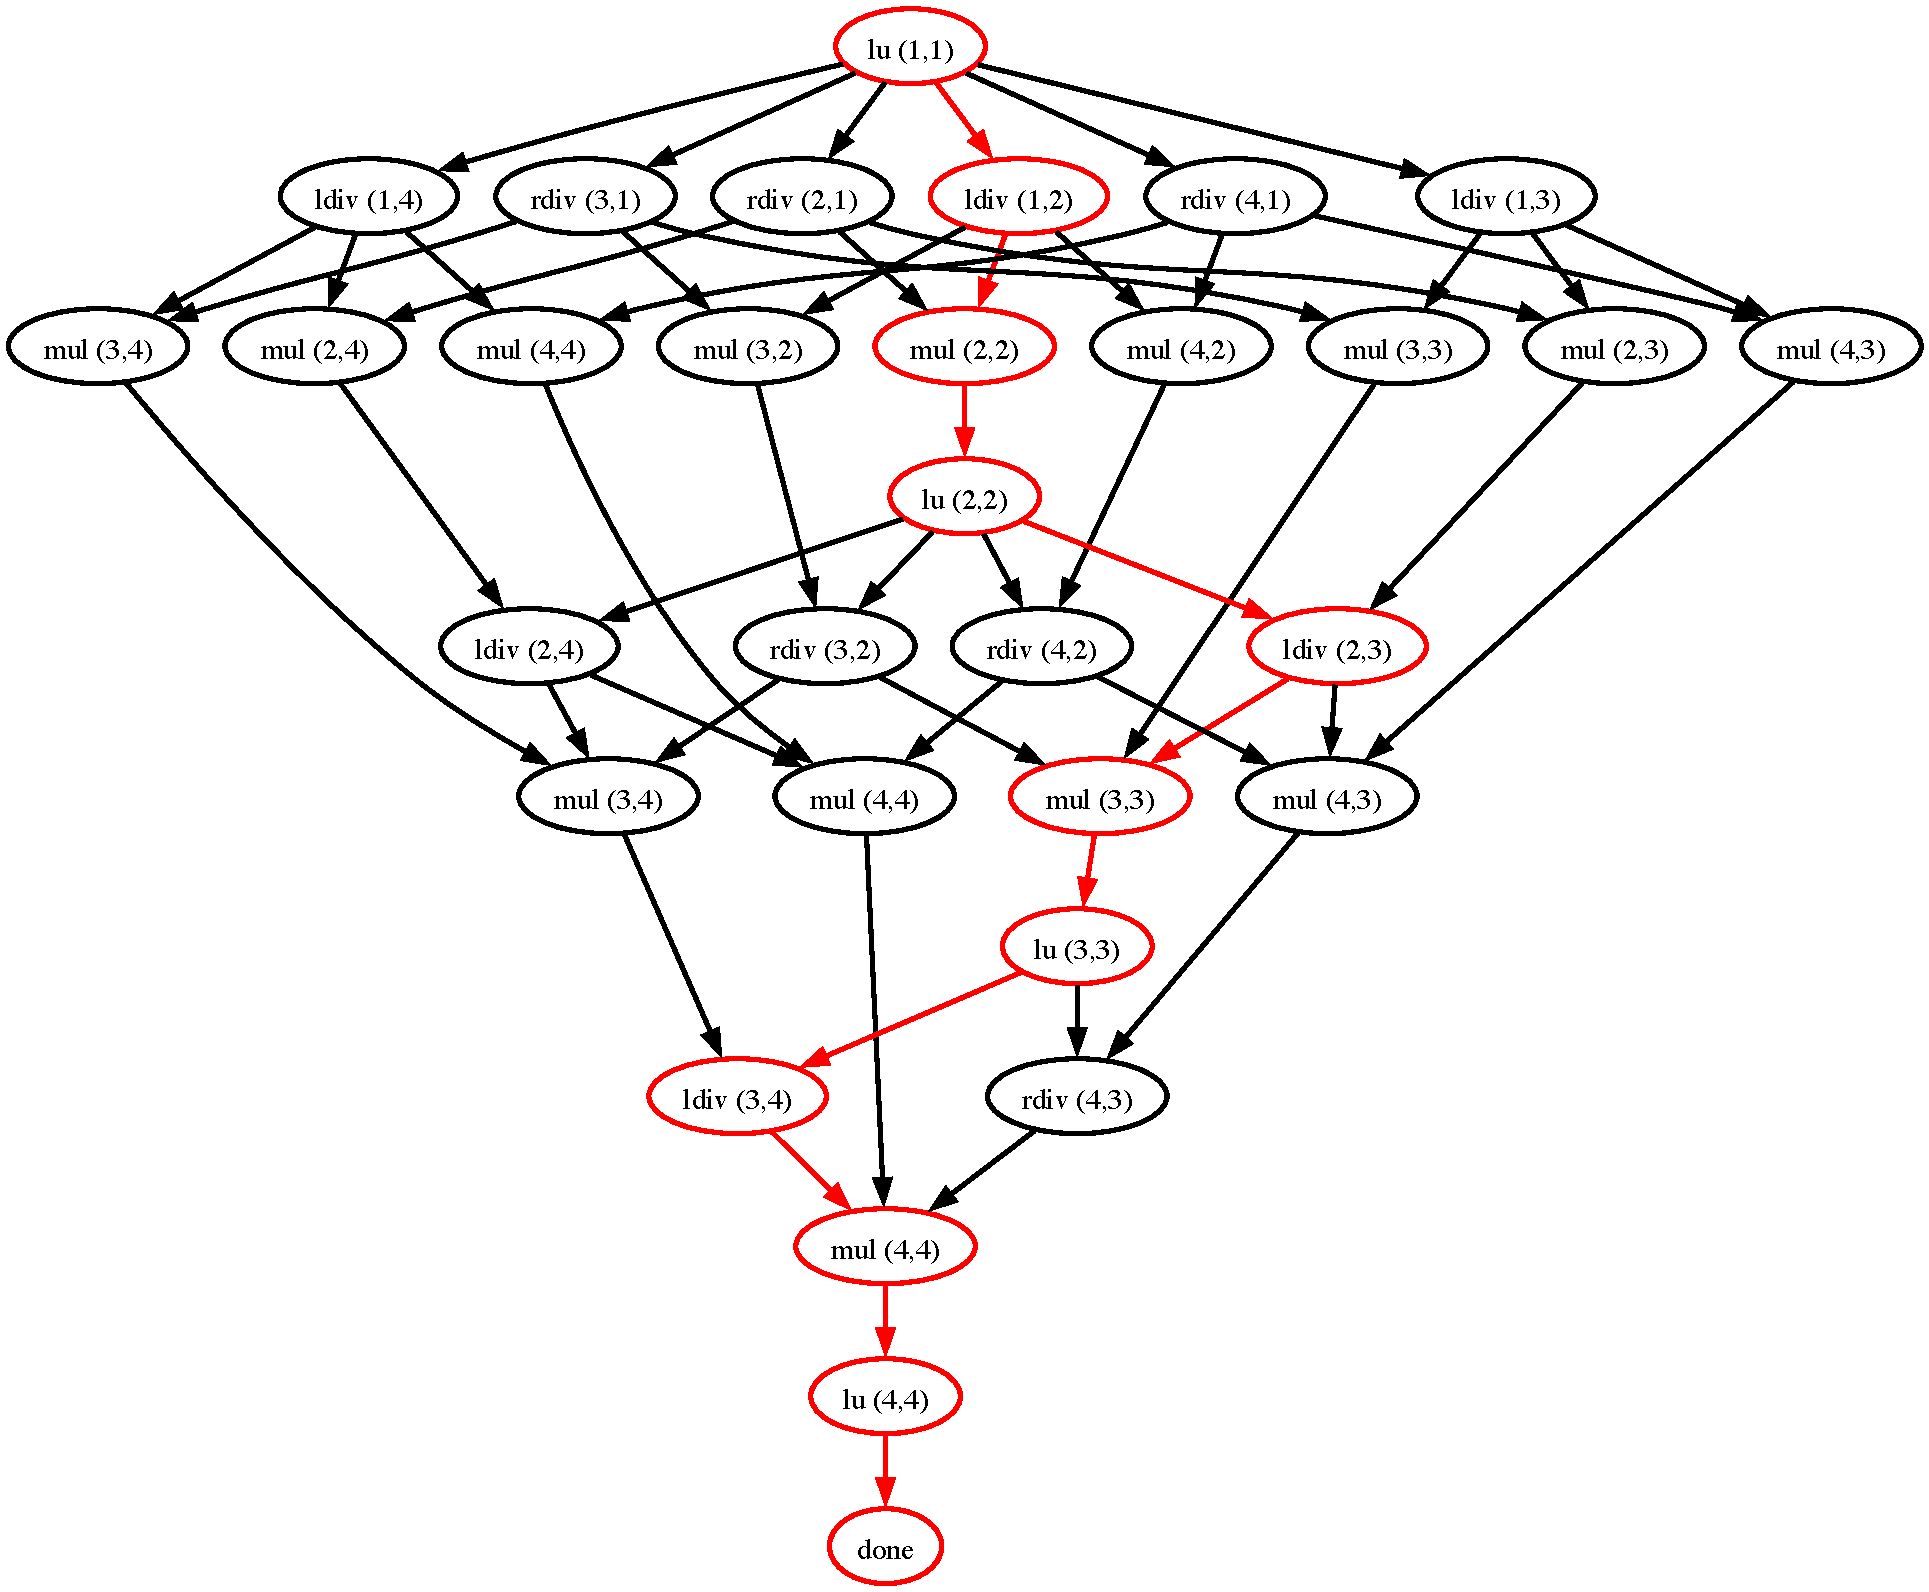
\includegraphics[width=\linewidth, height=0.72\textheight, keepaspectratio]{lu-dag.pdf}
		\end{column}
	\end{columns}

	\livedemo{lu_profile.jl}
\end{frame}

% ---------------------------------------------------------------------------
\begin{frame}[fragile]
	\frametitle{Profiling: the trace}
	\begin{minted}{julia}
using GLMakie  # interactive; CairoMakie: static
plot(log_info; categories = ["lu", "ldiv", "rdiv", "mul"])
	\end{minted}
	\centering
	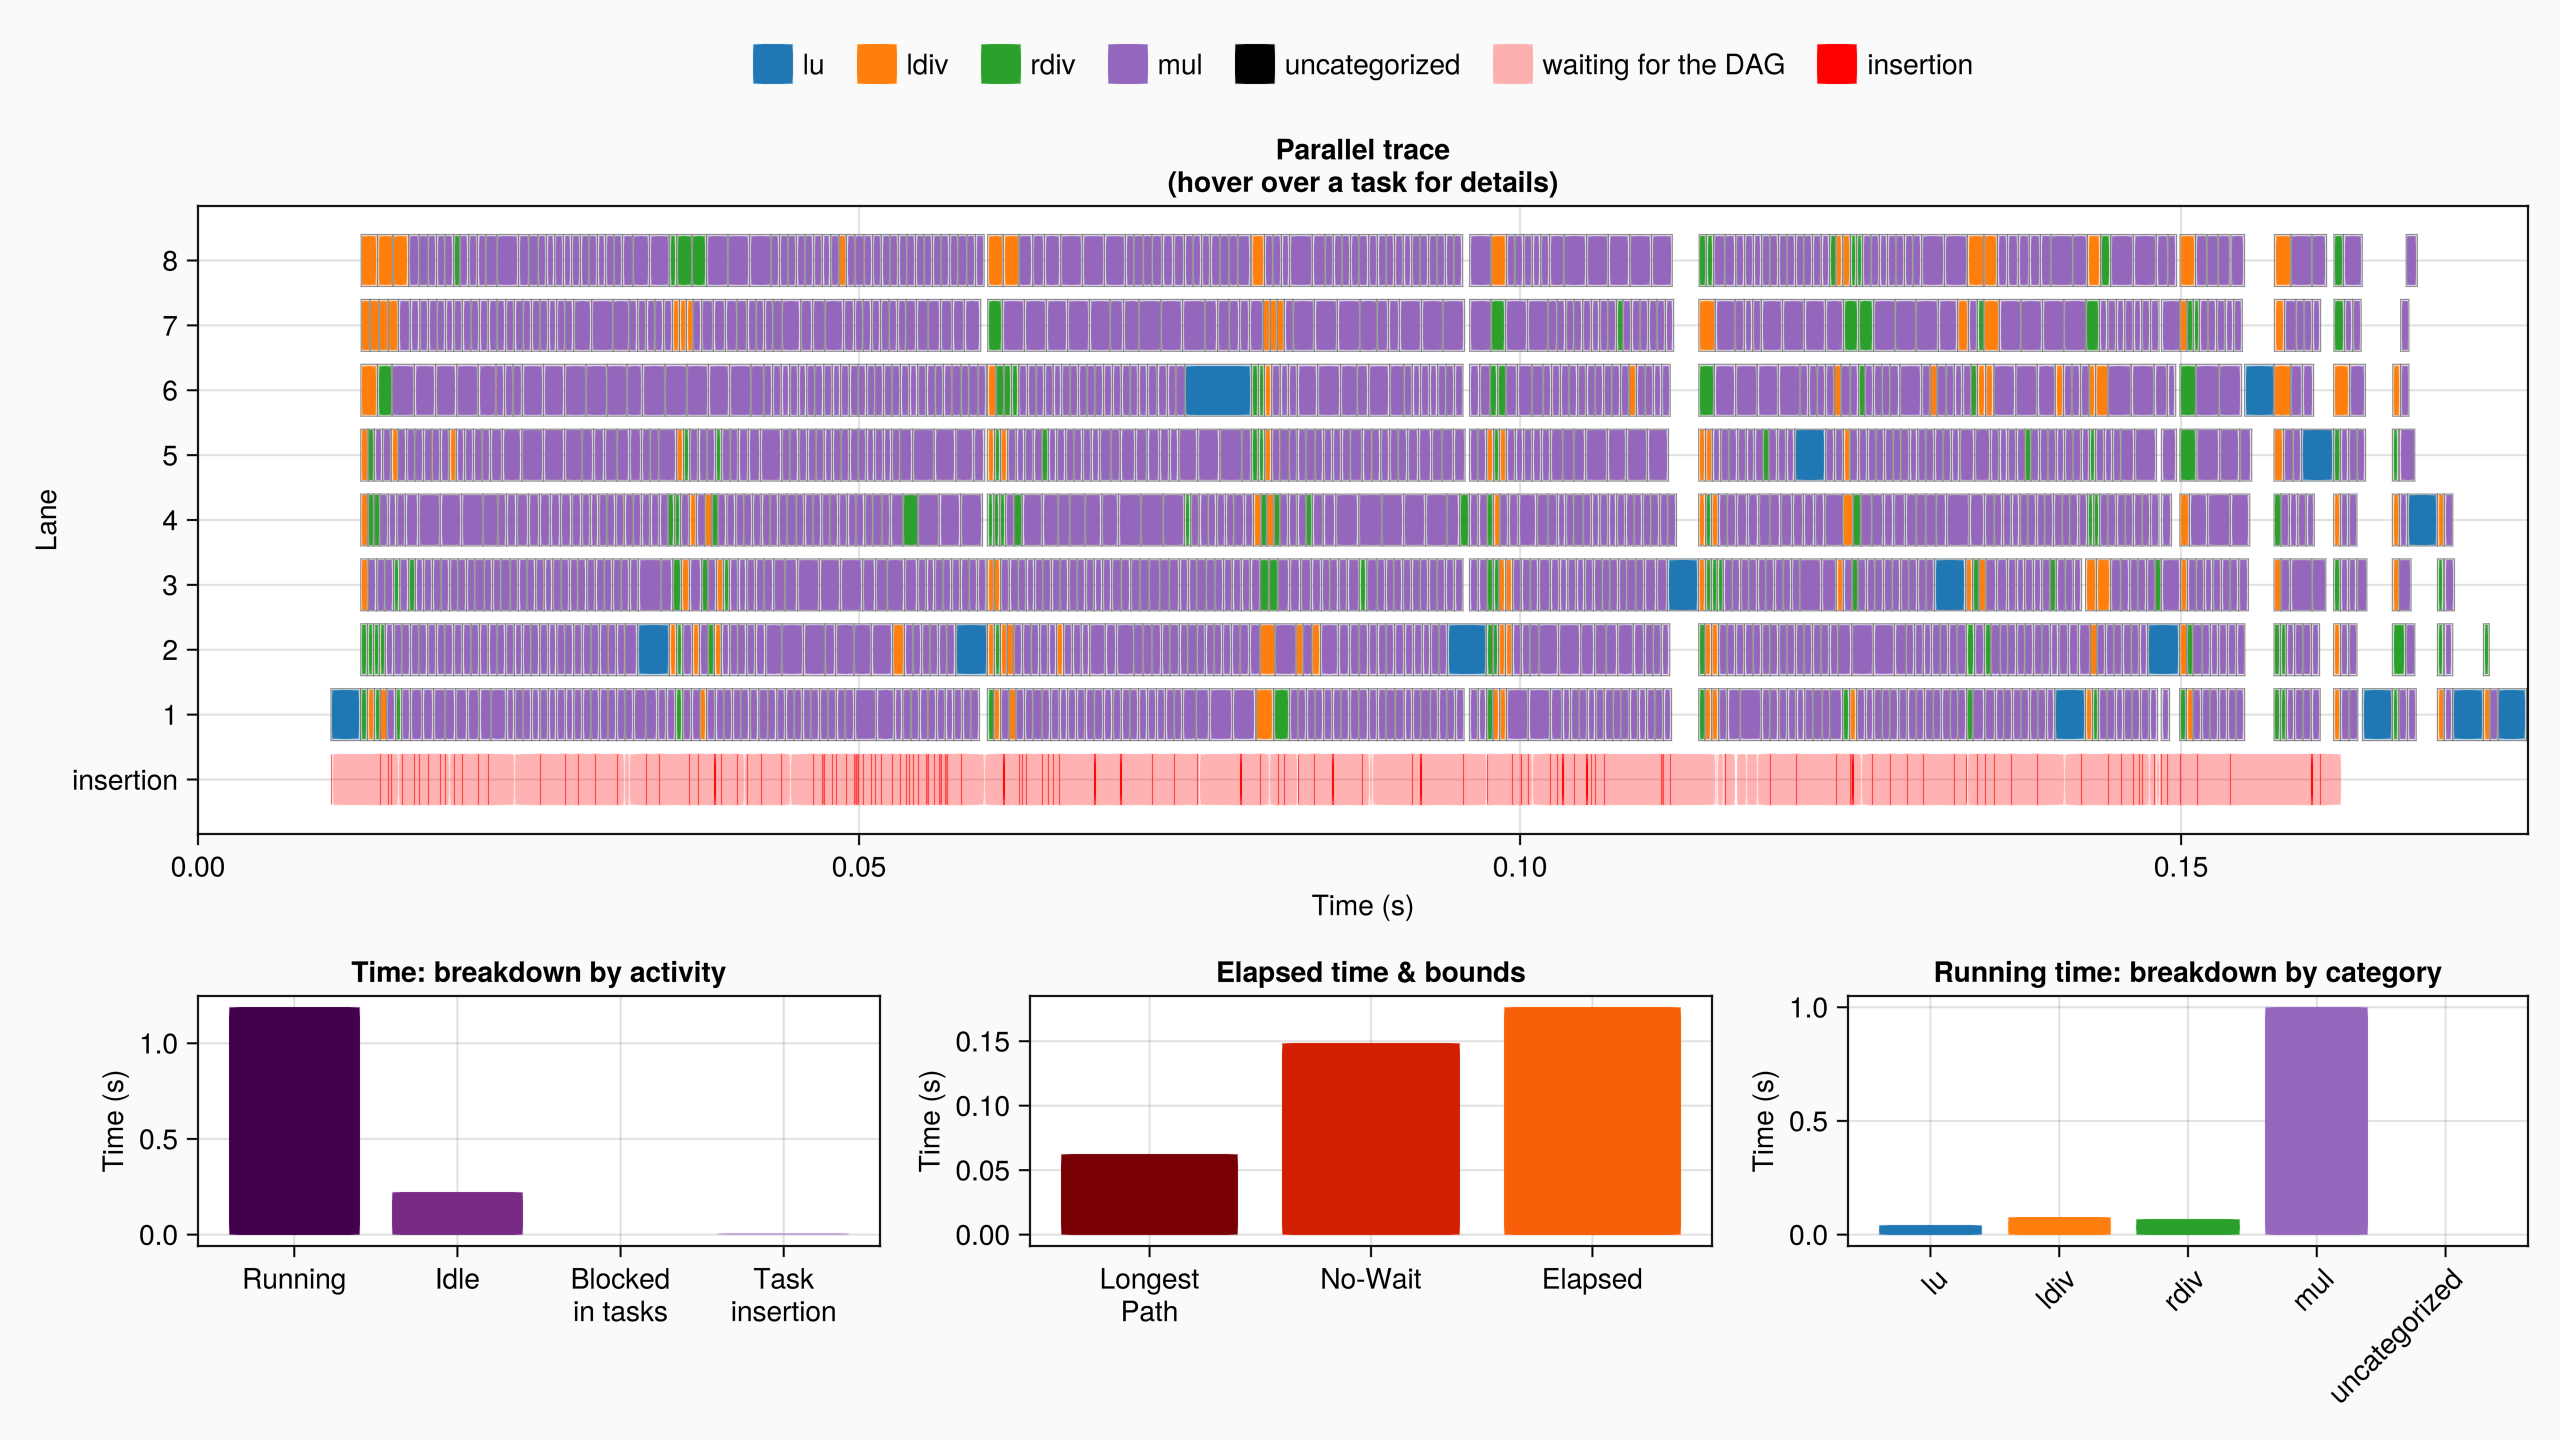
\includegraphics[width=\textwidth, trim=0 379 0 0, clip]{lu-trace.png}% top: the parallel trace

	\raggedright\small
	\begin{itemize}
		\item One bar per task, colored by category; one lane per thread
		\item Bottom lane: insertion in the \texttt{DAG} (\alert{red}), waiting for room (pink)
		\item \alert{Live}: hover a task for its dependencies and lifecycle, zoom on the lanes
	\end{itemize}

	\livedemo{lu_profile.jl}
\end{frame}

% ---------------------------------------------------------------------------
\begin{frame}
	\frametitle{Tiled LU: results}
	\(4000\times4000\), 8 threads, time in s \hfill {\small Apple M3 Pro, \DFT{} 0.3}

	\medskip
	\centering\small
	\begin{tabular}{lccccc}
		tile size        & 500  & 250  & 200  & 125  & 100  \\
		\hline
		tiled (1 thread) & 0.92 & 0.86 & 0.85 & 0.93 & 0.89 \\
		fork-join        & 0.29 & 0.18 & 0.17 & 0.17 & 0.17 \\
		tasks by hand    & 0.25 & 0.16 & 0.15 & 0.17 & 0.20 \\
		\DFT             & 0.25 & 0.16 & 0.16 & 0.18 & 0.23 \\
	\end{tabular}

	{\footnotesize LAPACK \texttt{lu!} (with pivoting), 8 BLAS threads: 0.19 s}

	\medskip
	\raggedright\normalsize
	\begin{itemize}
		\item \textbf{Fork-join is strong}: \texttt{mul!} is 84\,\% of the work, and independent within a step
		\item \textbf{Tasks win} where barriers idle threads: lone \texttt{lu!}, few tiles per thread, many cores
		\item \textbf{\DFT}: same graph as by hand, derived from the \alert{sequential code}; small tiles \(\Rightarrow\) insertion cost
		\item \textbf{Tile size}: large \(\Rightarrow\) little parallelism; small \(\Rightarrow\) overhead
	\end{itemize}

	\livedemo{lu_table.jl}
\end{frame}

% ---------------------------------------------------------------------------
\begin{frame}[fragile]
	\frametitle{Pitfalls}
	\begin{itemize}
		\item \textbf{Annotations are a contract}: missing or wrong \(\Rightarrow\) data race, no warning
		\item \textbf{Data now, code later}: annotations are evaluated at \texttt{@dspawn}, the body when the task runs
		      \begin{minted}[fontsize=\footnotesize]{julia}
@dspawn step!(@W(V), @R(U))
U, V = V, U  # the task body may see the swapped names!
		      \end{minted}
		      \(\Rightarrow\) closures capture \alert{variables}, not values: \mbox{\texttt{let U = U, V = V}}
		\item \textbf{Granularity}: insertion cost \(\propto\) tasks in the graph \(\Rightarrow\) tasks of \(\gtrsim\) 100 \textmu s
		\item \textbf{Inside a task}: avoid nested threading (\texttt{BLAS.set\_num\_threads(1)})
	\end{itemize}
\end{frame}

% ---------------------------------------------------------------------------
\begin{frame}
	\frametitle{Concluding remarks}
	\begin{itemize}
		\item \DFT{} makes parallel programming easier for \emph{certain} algorithms
		\item Simple API: \texttt{@dspawn} + \texttt{@R}, \texttt{@W}, \texttt{@RW}
		\item \textbf{Use it for}: many \alert{dependent} tasks on shared data (tiles, blocks, \ldots)
		\item \textbf{Not for}: tiny tasks (insertion cost), or independent loops (\texttt{@threads})
	\end{itemize}

	\bigskip
	\punchline{\url{https://github.com/maltezfaria/DataFlowTasks.jl}}

	\bigskip
	\centering Next: \alert{your turn}
\end{frame}

\section{Hands-on}

% ---------------------------------------------------------------------------
\begin{frame}
	\frametitle{Hands-on: your call}
	\begin{columns}[T]
		\begin{column}{0.5\textwidth}
			\textbf{Explore the scripts} \textcolor{gray}{(\texttt{scripts/})}
			\small
			\begin{itemize}
				\item Part 1: \texttt{threads\_loop}, \texttt{buffers\_threads}, \texttt{accumulate}, \texttt{lu\_tiled}, \ldots
				\item Part 2: \texttt{lu\_dft}, \texttt{lu\_profile}
			\end{itemize}
			\normalsize
			\textbf{Try}
			\small
			\begin{itemize}
				\item More threads, other tile / chunk sizes
				\item Profile with \texttt{DFT.@log}: what limits the run?
				\item Priorities for the \texttt{lu!}s; Cholesky
			\end{itemize}
		\end{column}
		\begin{column}{0.48\textwidth}
			\textbf{Bring your own code}
			\small
			\begin{itemize}
				\item A loop to parallelize, buffers to manage
				\item A task graph to express with \texttt{@dspawn}
			\end{itemize}
			\normalsize
			\textbf{Or a project}
			\small
			\begin{itemize}
				\item DataFrames.jl: threaded \texttt{ByRow}
				\item SparseArrays.jl: threaded \texttt{sparse(I,J,V)}
				\item \texttt{@dspawn} on DataFrames pipelines
			\end{itemize}
		\end{column}
	\end{columns}

	\punchline{Ask questions, we are around!}
\end{frame}













% ---------------------------------------------------------------------------
\begin{frame}
	\frametitle{Take-home}
	\begin{itemize}
		\item Write \alert{tasks}, not threads: no \texttt{threadid()} bookkeeping
		\item Buffers belong to tasks: one per chunk, or borrowed from a pool
		\item Shared mutable state: avoid it (partial sums), or protect it (lock, atomic)
		\item Dependent tasks: express the dependencies, ideally \alert{from the data} (\DFT)
	\end{itemize}

	\vfill
	\begin{itemize}
		\item Material: \url{https://github.com/maltezfaria/2026-frejus}
		\item \DFT{} docs: \href{https://github.com/maltezfaria/DataFlowTasks.jl}{\texttt{github.com/maltezfaria/DataFlowTasks.jl}}
		\item Julia manual: \textit{Multi-Threading}, \textit{Asynchronous Programming}
	\end{itemize}

	\vfill
	\centering\Large Thank you!
\end{frame}

% ===========================================================================
\appendix

\begin{frame}[plain]
	\centering\Huge\color{structure} Backup slides
\end{frame}

% ---------------------------------------------------------------------------
\begin{frame}[label=backup-threads]
	\frametitle{Threads vs.\ cores: why the OS layer?}
	\begin{itemize}
		\item \textbf{Thread} = software (stack + registers); \textbf{core} = hardware
		      \begin{itemize}
			      \item OS can pause a thread, save its state, resume it on \alert{any} core
		      \end{itemize}
		      \medskip
		\item \alert{Many more threads than cores} (\(\sim\)1000s vs.\ \(\sim\)10)
		      \begin{itemize}
			      \item OS \alert{time-slices} and \alert{preempts} threads
			      \item programs need not know the number of cores
		      \end{itemize}
		      \medskip
		\item \textbf{Blocking is cheap}: thread waits on I/O \(\Rightarrow\) OS runs another one
		      \medskip
		\item \textbf{Only the kernel schedules onto cores}
		      \begin{itemize}
			      \item programs can only \emph{request} an affinity
			      \item HPC: \alert{pin} threads to cores (cache, NUMA)\\
			            \texttt{ThreadPinning.jl}, \texttt{JULIA\_EXCLUSIVE=1}
		      \end{itemize}
		      \medskip
		\item Hyperthreading (SMT): 1 physical core = 2 hardware threads
	\end{itemize}
\end{frame}

% ---------------------------------------------------------------------------
\begin{frame}[label=backup-tasks]
	\frametitle{Why tasks on top of threads?}
	\centering
	\renewcommand{\arraystretch}{1.3}
	\begin{tabular}{l l l}
		                   & \textbf{OS thread} & \textbf{Julia task}                                 \\
		\hline
		Scheduled by       & kernel             & Julia runtime (user space)                          \\
		Memory             & \(\sim\)MB stack   & \(\sim\)KB                                          \\
		Switch cost        & kernel call        & cheap (user space)                                  \\
		Interruption       & \alert{preemptive} & \alert{cooperative} (yield points)                  \\
		Reasonable number  & \(\sim\)\#cores    & \(10^3\)--\(10^6\)                                  \\
	\end{tabular}

	\vfill
	\raggedright
	\begin{itemize}
		\item \textbf{M:N scheduling}: M tasks on N threads (N \(\approx\) \#cores)
		\item Nested \texttt{@spawn} \(\Rightarrow\) more tasks, \alert{not} more threads
		\item Task switches only at \texttt{wait}, \texttt{sleep}, I/O, \texttt{yield}, \ldots
		      \begin{itemize}
			      \item a busy loop keeps its thread
		      \end{itemize}
	\end{itemize}
\end{frame}

% ---------------------------------------------------------------------------
\begin{frame}[fragile, label=backup-atomic]
	\frametitle{Fix 2: atomic}
	\begin{minted}{julia}
ld = Atomic{Float64}(0.0)
@threads for i in 1:N
    F = lu(As[i])
    xs[i] = F \ bs[i]
    atomic_add!(ld, logdet(F))
end
ld[]  # read the value
	\end{minted}

	\vfill
	\begin{itemize}
		\item \alert{One} indivisible read-add-write: no lock object, no \texttt{Ref}
		\item Lower level: a hardware operation, not a task-level lock
		\item Only \alert{primitive types}: \texttt{Int}, \texttt{Float64}, \ldots
		\item Correct, same speed: \(0.47\,\text{s}\) (\texttt{-t 4})
		\item Lock or atomic: order of additions varies \(\Rightarrow\) \alert{last digit} varies
	\end{itemize}

	\livedemo{accumulate.jl}
\end{frame}

% ---------------------------------------------------------------------------
\begin{frame}[fragile, label=backup-partial]
	\frametitle{Also fine: partial sums}
	\begin{minted}{julia}
ts = map(partition(1:N, n)) do idxs
    @spawn begin
        s = 0.0
        for i in idxs
            F = lu(As[i])
            xs[i] = F \ bs[i]
            s += logdet(F)
        end
        s  # returned by the task
    end
end
ld = sum(fetch.(ts))
	\end{minted}

	\vfill
	\begin{itemize}
		\item The \alert{chunk pattern} again: no shared state, \texttt{fetch} returns it
		\item Same order every run \(\Rightarrow\) same digits
	\end{itemize}

	\livedemo{accumulate.jl}
\end{frame}

% ---------------------------------------------------------------------------
\begin{frame}
	\frametitle{Example: longest common subsequence (LCS)}
	\textbf{Subsequence}: same order, gaps allowed \hfill \texttt{diff}, DNA alignment, \ldots

	\medskip
	\(x = \texttt{GAC}\), \(y = \texttt{AGCAT}\) \(\Rightarrow\) LCS \(=\) \texttt{GA} or \texttt{AC}, length \alert{2}

	\vfill
	\begin{columns}[c]
		\begin{column}{0.45\textwidth}
			\centering
			\begin{tikzpicture}[x=0.55cm, y=0.55cm, font=\small,
					cell/.style={draw=gray!50, minimum size=0.55cm, inner sep=0pt},
					hd/.style={font=\small\ttfamily\bfseries, text=structure}]
				\foreach \c [count=\j from 0] in {\(\varnothing\),A,G,C,A,T} {\node[hd] at (\j,1) {\c};}
				\foreach \c [count=\i from 0] in {\(\varnothing\),G,A,C} {\node[hd] at (-1,-\i) {\c};}
		\node[cell] at (0,0) {0};
		\node[cell] at (1,0) {0};
		\node[cell] at (2,0) {0};
		\node[cell] at (3,0) {0};
		\node[cell] at (4,0) {0};
		\node[cell] at (5,0) {0};
		\node[cell] at (0,-1) {0};
		\node[cell] at (1,-1) {0};
		\node[cell] at (2,-1) {1};
		\node[cell] at (3,-1) {1};
		\node[cell] at (4,-1) {1};
		\node[cell] at (5,-1) {1};
		\node[cell] at (0,-2) {0};
		\node[cell] at (1,-2) {1};
		\node[cell] at (2,-2) {1};
		\node[cell] at (3,-2) {1};
		\node[cell] at (4,-2) {2};
		\node[cell] at (5,-2) {2};
		\node[cell] at (0,-3) {0};
		\node[cell] at (1,-3) {1};
		\node[cell] at (2,-3) {1};
		\node[cell] at (3,-3) {2};
		\node[cell] at (4,-3) {2};
		\node[cell] at (5,-3) {2};
				% dependencies of cell (C, C)
				\node[cell, fill=orange!40] at (3,-3) {2};
				\node[cell, fill=blue!15] at (2,-2) {1};
				\node[cell, fill=gray!15] at (3,-2) {1};
				\node[cell, fill=gray!15] at (2,-3) {1};
			\end{tikzpicture}

			\scriptsize \colorbox{orange!40}{C = C} \(\Rightarrow\) \colorbox{blue!15}{diagonal} \(+\,1\)
		\end{column}
		\begin{column}{0.53\textwidth}
			\(L_{ij}\) = LCS length of \(x_{1:i}\) and \(y_{1:j}\):
			\[
				L_{ij} =
				\begin{cases}
					L_{i-1,j-1} + 1                    & x_i = y_j \\
					\max(L_{i-1,j},\, L_{i,j-1})       & \text{otherwise}
				\end{cases}
			\]
			\begin{itemize}
				\item First row and column: \(0\)
				\item Answer: \(L_{\text{end},\text{end}}\), then backtrack
				\item Cost: \(O(|x|\,|y|)\)
			\end{itemize}
		\end{column}
	\end{columns}
\end{frame}

% ---------------------------------------------------------------------------
\begin{frame}[fragile]
	\frametitle{LCS: why is it hard to parallelize?}
	\begin{columns}[c]
		\column{0.36\textwidth}
		\centering
		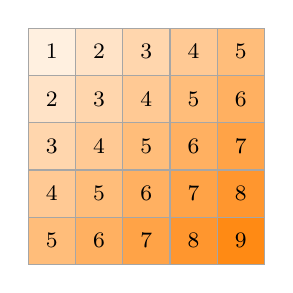
\begin{tikzpicture}[x=0.6cm, y=0.6cm, font=\footnotesize,
				tile/.style={draw=gray!70, minimum size=0.6cm, inner sep=0pt}]
				\node[tile, fill=orange!12] at (0,0) {1};
				\node[tile, fill=orange!22] at (1,0) {2};
				\node[tile, fill=orange!32] at (2,0) {3};
				\node[tile, fill=orange!42] at (3,0) {4};
				\node[tile, fill=orange!52] at (4,0) {5};
				\node[tile, fill=orange!22] at (0,-1) {2};
				\node[tile, fill=orange!32] at (1,-1) {3};
				\node[tile, fill=orange!42] at (2,-1) {4};
				\node[tile, fill=orange!52] at (3,-1) {5};
				\node[tile, fill=orange!62] at (4,-1) {6};
				\node[tile, fill=orange!32] at (0,-2) {3};
				\node[tile, fill=orange!42] at (1,-2) {4};
				\node[tile, fill=orange!52] at (2,-2) {5};
				\node[tile, fill=orange!62] at (3,-2) {6};
				\node[tile, fill=orange!72] at (4,-2) {7};
				\node[tile, fill=orange!42] at (0,-3) {4};
				\node[tile, fill=orange!52] at (1,-3) {5};
				\node[tile, fill=orange!62] at (2,-3) {6};
				\node[tile, fill=orange!72] at (3,-3) {7};
				\node[tile, fill=orange!82] at (4,-3) {8};
				\node[tile, fill=orange!52] at (0,-4) {5};
				\node[tile, fill=orange!62] at (1,-4) {6};
				\node[tile, fill=orange!72] at (2,-4) {7};
				\node[tile, fill=orange!82] at (3,-4) {8};
				\node[tile, fill=orange!92] at (4,-4) {9};
		\end{tikzpicture}

		\smallskip
		\scriptsize tiles, numbered by \alert{step}: a \alert{wavefront}

		\column{0.62\textwidth}
		\begin{itemize}
			\item Cell needs top, left, diagonal: rows not independent, \texttt{@threads} \xmark
			\item Anti-diagonals are, but a cell is one comparison
			\item \alert{Tiles}: \((i,j)\) needs \((i-1,j)\) and \((i,j-1)\)
		\end{itemize}

		\medskip
		By hand (Part~1):
		\begin{minted}[fontsize=\scriptsize]{julia}
T = Matrix{Task}(undef, n, n)
for j in 1:n, i in 1:n
    T[i,j] = @spawn begin
        i > 1 && wait(T[i-1,j])
        j > 1 && wait(T[i,j-1])
        fill_lengths!(L, x, y, I[i], J[j])
    end
end
		\end{minted}
	\end{columns}

	\begin{itemize}
		\item Works, but \alert{you} derived the graph: indices, borders, init, \ldots
	\end{itemize}
\end{frame}

% ---------------------------------------------------------------------------
\begin{frame}[fragile]
	\frametitle{LCS with \DFT}
	\begin{columns}[T]
		\column{0.44\textwidth}
		\textbf{Tiled, sequential}
		\begin{minted}[fontsize=\scriptsize]{julia}
L[:, 1] .= 0
L[1, :] .= 0
for jr in J, ir in I

    fill_lengths!(L, x, y, ir, jr)


end
backtrack(L, x, y)
		\end{minted}

		\column{0.54\textwidth}
		\textbf{Parallel}
		\begin{minted}[fontsize=\scriptsize]{julia}
@dspawn fill!(@W(view(L, :, 1)), 0)
@dspawn fill!(@W(view(L, 1, :)), 0)
for jr in J, ir in I
    @dspawn begin
        @R view(L, ir, jr)
        @RW view(L, ir .+ 1, jr .+ 1)
        fill_lengths!(L, x, y, ir, jr)
    end
end
fetch(@dspawn backtrack(@R(L), x, y))
		\end{minted}
	\end{columns}

	\vfill
	\begin{itemize}
		\item Same loops (\texttt{I}, \texttt{J}: tiles); each tile says what it \alert{reads} and \alert{writes}
		\item Tile reads its top/left neighbors (overlap with \texttt{ir}, \texttt{jr}), writes itself
		\item The wavefront \alert{emerges} from the annotations
	\end{itemize}
\end{frame}

% ---------------------------------------------------------------------------
\begin{frame}[fragile]
	\frametitle{LCS: performance}
	\(x\), \(y\) of length \(8192\) and \(16384\); \(16\times16\) tiles

	\medskip
	\centering
	\begin{tabular}{lccc}
		                         & \texttt{-t 1} & \texttt{-t 4} & \texttt{-t 8} \\
		\hline
		sequential               & 0.10 s        & 0.10 s        & 0.10 s        \\
		tasks by hand (\texttt{wait}) & 0.12 s   & 0.042 s       & 0.029 s       \\
		\DFT                     & 0.12 s        & 0.043 s       & 0.033 s       \\
	\end{tabular}

	\vfill
	\raggedright
	\begin{itemize}
		\item Same speed as by hand, without deriving the graph
		\item \(\approx 3\times\) on 8 threads: memory-bound, and the wavefront must \alert{ramp up}
		\item Too many tiles (\(64\times64\)): \alert{slower}, task overhead dominates
	\end{itemize}

	\livedemo{lcs.jl}
\end{frame}

% ---------------------------------------------------------------------------
\begin{frame}[label=backup-lu-algorithm]
	\frametitle{Tiled LU: the algorithm}
	The \(2\times2\) block LU of Part~1, applied tile by tile:

	\medskip
	\begin{columns}[c]
		\column{0.36\textwidth}
		\centering
		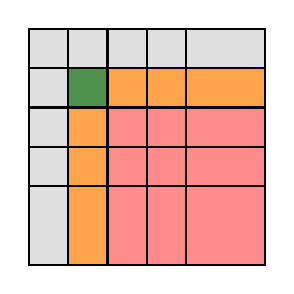
\begin{tikzpicture}[scale=0.5, thick]
			\pic[fill=gray!25] at (0,-1) {square};
			\pic[fill=gray!25] at (1,-1) {square};
			\pic[fill=gray!25] at (2,-1) {square};
			\pic[fill=gray!25] at (3,-1) {square};
			\pic[fill=gray!25] at (4,-1) {square};
			\pic[fill=gray!25] at (0,-2) {square};
			\pic[fill=themegreen!70] at (1,-2) {square};
			\pic[fill=orange!70] at (2,-2) {square};
			\pic[fill=orange!70] at (3,-2) {square};
			\pic[fill=orange!70] at (4,-2) {square};
			\pic[fill=gray!25] at (0,-3) {square};
			\pic[fill=orange!70] at (1,-3) {square};
			\pic[fill=red!45] at (2,-3) {square};
			\pic[fill=red!45] at (3,-3) {square};
			\pic[fill=red!45] at (4,-3) {square};
			\pic[fill=gray!25] at (0,-4) {square};
			\pic[fill=orange!70] at (1,-4) {square};
			\pic[fill=red!45] at (2,-4) {square};
			\pic[fill=red!45] at (3,-4) {square};
			\pic[fill=red!45] at (4,-4) {square};
			\pic[fill=gray!25] at (0,-5) {square};
			\pic[fill=orange!70] at (1,-5) {square};
			\pic[fill=red!45] at (2,-5) {square};
			\pic[fill=red!45] at (3,-5) {square};
			\pic[fill=red!45] at (4,-5) {square};
		\end{tikzpicture}

		\scriptsize step \(k = 2\) of \(5\)

		\column{0.62\textwidth}
		\texttt{for k in 1:n}
		\begin{enumerate}
			\item \textcolor{themegreen}{diagonal}: \(T_{kk} \leftarrow L_{kk}U_{kk}\) \hfill \texttt{lu!}
			\item \textcolor{orange}{row panel}: \(T_{kj} \leftarrow L_{kk}^{-1}T_{kj}\) \hfill \texttt{ldiv!}
			\item[] \textcolor{orange}{column panel}: \(T_{ik} \leftarrow T_{ik}U_{kk}^{-1}\) \hfill \texttt{rdiv!}
			\item \textcolor{red}{trailing update}: \(T_{ij} \leftarrow T_{ij} - T_{ik}T_{kj}\) \hfill \texttt{mul!}
		\end{enumerate}
	\end{columns}

	\vfill
	\begin{itemize}
		\item \(O(n)\) \texttt{lu!}, \(O(n^2)\) \texttt{ldiv!}/\texttt{rdiv!}, \(O(n^3)\) \texttt{mul!}: compute-bound
		\item \textcolor{gray}{Gray}: done. In place: \(L\) and \(U\) overwrite \(A\)
	\end{itemize}
\end{frame}

\end{document}

%%% Local Variables:
%%% mode: LaTeX
%%% TeX-master: t
%%% End:
